%% Copernicus Publications Manuscript Preparation Template for LaTeX Submissions
%% ---------------------------------
%% This template should be used for the following class files: copernicus.cls, copernicus2.cls, copernicus_discussions.cls
%% The class files, the Copernicus LaTeX Manual with detailed explanations regarding the comments
%% and some style files are bundled in the Copernicus Latex Package which can be downloaded from the different journal webpages.
%% For further assistance please contact the Publication Production Office (production@copernicus.org).
%% http://publications.copernicus.org


%% Differing comments regarding the specific class files are highlighted.

%% copernicus.cls
\documentclass[journal abbreviation]{copernicus}

%% copernicus2.cls
%\documentclass[journal abbreviation]{copernicus2}

%% copernicus_discussions.cls
%\documentclass[journal abbreviation, hvmath, online]{copernicus_discussions}

%bibtex
\bibliographystyle{copernicus}


\begin{document}


\title{Early decomposition lignin degradation depends on nutrient availability in beech litter}


\author[1]{Lukas Kohl}
\author[1]{Maria Mooshammer}
\author[1]{Sonja Leitner}
\author[1]{Ieda H\"ammerle-N.}
\author[1]{Alexander Frank}
\author[1]{Lucia Fuchslueger}
\author[1]{J\"org Schnecker}
\author[2]{Katherina Keiblinger}
\author[2]{Sophie Zechmeister-Bolkenstein}
\author[1]{Wolfgang Wanek}
\author[1]{Andreas Richter}



\affil[1]{Checo}
\affil[2]{BFW}


%% The [] brackets identify the author to the corresponding affiliation, 1, 2, 3, etc. should be inserted.b



\runningtitle{TEXT}

\runningauthor{TEXT}
 
\correspondence{me.\\ (email@here.at)}
%check with wolfi


\received{}
\pubdiscuss{} %% only important for two-stage journals
\revised{}
\accepted{}
\published{}
%% These dates will be inserted by the Publication Production ffice during the typesetting process. 


\firstpage{1}

\maketitle



\begin{abstract}
TEXT
\end{abstract}


%% only used for copernicus2.cls
%\abstract{
% TEXT
% \keywords{TEXT}}

\introduction
\section{General Information}

This document is intended as a template and guideline and should support the author in the course of doing the master's thesis.
Assessment criteria comprise the quality of the theoretical and/or practical work as well as structure, content and wording of the written master's thesis. Careful attention should be given to the basics of scientific work (e.g., correct citation).

\section{Organizational Issues}

A master's thesis at the Faculty of Informatics has to be finished within six months. During this period regular meetings between the advisor(s) and the author have to take place.
In addition, the following milestones have to be fulfilled:
\begin{enumerate}
  \item  Within one month after having fixed the topic of the thesis the master's thesis proposal has to be prepared and must be accepted by the advisor(s). The master's thesis proposal must follow the respective template of the dean of academic affairs. Thereafter the proposal has to be applied for at the deanery. The necessary forms may be found on the web site of the Faculty of Informatics. \url{http://www.informatik.tuwien.ac.at/dekanat/formulare.html}
  \item  Accompanied with the master's thesis proposal, the structure of the thesis in terms of a table of contents has to be provided.
  \item Then, the first talk has to be given at the so-called ``Seminar for Master Students''. The slides have to be discussed with the advisor(s) one week in advance. Attendance of the ``Seminar for Master Students'' is compulsory and offers the opportunity to discuss arising problems among other master students.
  \item At the latest five months after the beginning, a provisional final version of the thesis has to be handed over to the advisor(s).  
  \item As soon as the provisional final version exists, a first poster draft has to be made. The making of a poster is a compulsory part of the ``Seminar for Master Students'' for all master studies at the Faculty of Informatics. Drafts and design guidelines can be found at \url{http://www.informatik.tuwien.ac.at/studium/richtlinien}.
  \item After having consulted the advisor(s) the second talk has to be held at the ``Seminar for Master Students''.
  \item At the latest six months after the beginning, the corrected version of the master's thesis and the poster have to be handed over to the advisor(s).
  \item After completion the master's thesis has to be presented at the ``epilog''. For detailed information on the epilog see: \\ \url{http://www.informatik.tuwien.ac.at/studium/epilog}
\end{enumerate}

\section{Structure of the Master's Thesis}

If the curriculum regulates the language of the master's thesis to be English (like for ``Business Informatics''), the thesis has to be written in English. Otherwise, the master's thesis may be written in English or in German. The structure of the thesis is predetermined.
The table of contents is followed by the introduction and the main part, which can vary according to the content. The master's thesis ends with the bibliography (compulsory) and the appendix (optional).

\begin{itemize}
  \item	Cover page
  \item Acknowledgements
  \item Abstract of the thesis in English and German
  \item Table of contents
  \item Introduction
  	\begin{itemize}
  		\item motivation
  		\item problem statement (which problem should be solved?)
  		\item aim of the work
  		\item methodological approach
  		\item structure of the work
  	\end{itemize}
  \item State of the art / analysis of existing approaches
  	\begin{itemize}
  		\item literature studies
  		\item analysis
  		\item comparison and summary of existing approaches
  	\end{itemize}
  \item Methodology
  	\begin{itemize}
  		\item used concepts
  		\item methods and/or models
  		\item languages
  		\item design methods
  		\item data models
  		\item analysis methods
  		\item formalisms
  	\end{itemize}
  \item Suggested solution/implementation
  \item Critical reflection
  	\begin{itemize}
  		\item comparison with related work
  		\item discussion of open issues
  	\end{itemize}
  \item Summary and future work
  \item Appendix: source code, data models, \dots
  \item Bibliography
\end{itemize}


\section{Material and methods}

\subsection{Litter decomposition experiment}
A detailed description of our litter decomposition experiment was published in \cite{Wanek2011}. Briefly, beech litter from four sites in Austria (Achenkirch (AK), Klausenleopoldsdorf(KL), Ossiach(OS), and Schottenwald(SW); refered to as litter types) was collected in October 2008. Litter was homogenized, sterilized and inoculated (1.5\% w/w) with a mixture of litter and soil to assure all litter types share the same initial microbial community. From each type, four samples of  litter were taken after inoculation.
Samples of 60g litter (fresh weight) were kept at 15 \textdegree C and 60\% water content in mesocosms for a duration between 2 weeks to 15 month. For each litter type 5 replicas were removed and analyzed after 14, 97, 181 and 375 days. 

\subsection{Bulk litter, extractable, and microbial biomass nutrient content}
To calculate litter mass loss, litter dry mass content was measurement in 5 g litter (fresh weight) after 48 h at 80 \textdegree C. Dried litter was ball-milled for further chemical analysis. Litter C and N content were determined using an elemental analyzer (Leco CN2000, Leco Corp., St. Joseph, MI, USA). Litter phosphorus content was measured  with ICP-AES (Vista-Pro, Varian, Darmstadt, Germany) after acid digestion as described by \cite{Henschler1988}.

To determine soluble C, N, and P contents, 1.8g litter (fresh weight) were extracted with 50 ml 0.5M K\textsubscript{2}SO\textsubscript{4}. Samples were shaken on a reciprocal shaker with the extractant for 30 minutes, filtered with ash-free filters and frozen at -20 \textdegree C until analysis. For quantifying microbial biomass C, N and P pools, the same extraction was used after chloroform fumigation . Microbial biomass was determined as the difference between fumigated and non-fumigated extractions. C and N concentration in extracts were determined with a TOC/TN analyzer (TOC-VCPH and TNM, Schimadzu), Phosphorous was determined photometrically [..] [lit: schinner 1996]

Substrate-consumer stoichiometric inbalances \emph{X:Y$_{inbal}$} were calculated as

 \begin{equation}
X:Y_{inbal}=\frac{X:Y_{litter}}{X:Y_{microbial}} \label{eq:resp.acc}
 \end{equation}

where \emph{X} and \emph{Y} stand for on of the elements C, N, or P.

\subsection{Microbial Respiration}
Respiration was monitored weekly in the mesocosms that were harvested after 181 month and for all mesocosms one days before the harvestg an infrared gas analyzer (IRGA, EGM4 with SRC1, PPSystems, USA). CO2 concentration was measured over 70 seconds and increase per second was calculated based on g dry weight of the litter. Measurements of ambient air were performed before and after each measurement to assess possible leaks or base-line drifts IRGA. %Measurements were conducted using the following settings: volume of the chamber 1551 cm³, area of the chamber 115 cm², linear measurement, at 15\textdegree.
Accumulated respiration after 181 month was calculated assuming linear transition between measurements, accumulated respiration after 475 days was estimated from respiration rates after 181 and 475 days. We do not base interpretation exclusively on the later estimate but use is mainly ..
%as stated in equation \ref{eq:resp.acc}, where \emph{Resp\textsubscript{acc}} stands for the accumulated respiration, \emph{Resp\textsubscript{n}} and \emph{t\textsubscript{n}} for the actual respiration at and the decomposition time until time point \emph{n}.

% \begin{equation}
% Resp_{acc}(t_{n})=\sum_{i=0}^n (Resp(t_{i})+Resp(t_{i+1}))*(t_{i+1}-t_{i})/2
% \label{eq:resp.acc}
% \end{equation}

\subsection{Enzyme activities}

Measurements of potential exo-enzyme activities for cellulases, peroxidases and phenoloxidase were described by \cite{Leitner2011}. Activities were determined with a series of micro-plate assays based on the hydrolysis of 4-methyl-$\beta$-D-cellobioside (cellulase) and L-3,4-di\-hydroxy\-phenyl\-alanin (oxidative enzymes). Products of enzyme catalyzed reactions were detected photometrically (oxidative enzymes) or flourometrically (cellulase). The method was was initially published by \cite{Marx2001} and \cite{Sinsabaugh1999}, we applied a modified variant as described in \cite{Kaiser2010b}. Enzyme activity was measured after 14, 87 and 181 days. In this study we use the quotient between cellulase and oxidative enzymes to describe litter microorganisms investments in the trade-off lignin and cellulose degradation. 

\subsection{Glucan depolymerization and carbon use efficiency}
Glucan depolymerization and Glucose consumption were measured by \cite{Leitner2011} after 14, 97, and 181 days using a new 13C pooldillution assay . Method and results were reported in \cite{Leitner2011}. Based on the their results, we calculated the carbon use efficiency \emph{CUE} based on g carbon metabolized:

\begin{equation}
CUE = (\frac{Glucose Consumption - Respiration}{Respiration})
\end{equation}

\subsection{Metaproteome (and Metatranscriptome?) analysis}
...

\subsection{Pyrolysis-GC/MS}
Pyrolysis-GC/MS was performed on a Pyroprobe 5250 pyrolysis system (CDS Analytical) coupled to a Thermo Trace gas chromatograph and a DSQ II MS detector (both Thermo Scientific) equipped with a carbowax colomn (Supelcowax 10, Sigma-Aldrich).

Litter analyzed was sampled immediately after inoculation and after 97, 181, and 375 days. 2-300 \textmu g dried and finely ball-milled litter were heated to 600\textdegree C for 10 seconds in helium atmosphere. The temperature of the valve oven and the transfer line to the GC injection port were set to 250\textdegree C,a 10x split injection was applied with the injector heated to 240\textdegree C. GC Oven temperature was constant at 50 \textdegree C for 2 minutes, followed by an increase of 7\textdegree C/min to a final temperature of 260 \textdegree C, which was held for 15 minutes. The transfer line was heated to 270 \textdegree C. The MS detector was set for electron ionization at 70 EV, the ion source was heated to 270\textdegree C. Detection was set to cycle between m/z 20 and 300 with a cycle time of 0.3 seconds.

Peaks were assignment was based on NiSt 05 MS library and comparison with reference material measured. 133 peaks were identified and selected for integration due to their hight abundance or diagnostic value. For each peak between one and four dominant mass fragments selected for high abundance and specificity were integrated (as done by i.e. \cite{Schellekens2009}). Peak areas are stated as \% of the sum of all integrated peaks of a sample. 

Pyrolysis products were assigned to their substances of origin by comparison to reference material, structural similarity and in accordance with literature (\cite{Ralph1991a, Schellekens2009,Chiavari1992}[more lit!]). The sum of all peak areas of the pyrolysis products of a class was calculated based on total ion current (TIC) peak areas. TIC peak areas are (1) less specific as areas of specific MS fragments and (2) integration was not possible for all peaks a/o all samples. Therefore a MS response factor Rf was calculated for each detected substance:

\begin{equation}
Rf = median (\frac{TIC peak area}{specific MS fragment peak area})
\end{equation}

Peak areas were multiplied by Rf before addition to calculate percentages of TIC area without loosing the specifity of integrating single m/z traces.

% However, during interpretation, we found little difference between direct sums of the integrated fragments and sums of corrected areas, indicating little sensitivity for exact 

Relative peak areas in both integrations are different from weight\%, but allow tracing of accumulation/depletion of these substance classes during decomposition \citep{Schellekens2009}. 

%check pyridol peak!!

%All nitrogen containing compounds and their sum were correlated to litter N content (R\textgreater0.49 for all  and R\textgreater0.79 for 8 of 11 pyrolysis products and the sum of all N containing compounds. For all correlations, p=***). all peaks were correlated to their sum with .... The cTIC sum correlated to PCA1 with R\textgreater0.8x (p=***=).

%Of the 28 lignin derived molecules were detected, 26 were positivly correlated to their sum (p=** or ***), 18 with R\textgreater0.07 (all p=***). Another the 10 non-lignin phenolic compounds found, of which 9 were positively correlated to the sum of all Phenoles, 7 with R\textgreater0.7.

\subsection{Statistical analysis}
All statistical analyses were performed with the software and statistical computing environment R using the R package ``vegan'' \citep{Oksanen2011}. If not mentioned otherwise, results were considered significant, when p\textless 0.05. All correlations refer to Pearson correlations.
All data presented was tested for significant differences between harvests and litter types. Normal distribution assumed but could not be tested due to the small number of cases per treatment (n=4-5). A substantial part of variables had heterogeneous variances when tested ẃith Levene's test. Therefore, (one-way) Welch anova was used to calculate significant differences between harvests within each litter type and litter types within each harvest (alpha=0.05). For post-hoc group assignment, paired Welch's t-tests with Bonferroni corrected p limits were used. Principal component analysis was performed using vegan function ``rda'' scaling variables.

\section{Results}
\subsection{Litter stoichiometry and micronutrient content}

The chemical characteristics of the four litter types was previously reported by \cite{Wanek2011}. Initial Macro- and Micro-nutrient content of litter are presented in figure \ref{fig:litchem_h1}, table \ref{tab:summary} gives a summary of differences between litter types. Mean initial C:N ratios were between 1:41 and 1:58, initial C:P ratios between 1:700 and 1:1300. Initial N:P ratios ranged between 1:15 and 1:30. No significant changes occurred during litter incubation except a slight decrease of the C:N ratio (1:41.8 to 1:37.4) found in the most active litter type (SW) after 15 month.

Fe content were more than twice as high for OS (approx. 450 ppm) than for other litter types (approx. 200 ppm). Litter Mn also was highly variable between litter types, ranging between 170 and 2130 ppm. Litter Mn content was negatively correlated to N ratio [stat]. Changes of micro-nutrient concentrations during litter incubation were significant, but in all cases \textless 15\% of the initial concentration.

Soluble organic carbon content decreased between the first three harvests (14 to 181 days), to strongly increase after 375 days. Contents ranged between 0.1 and 0.7 mg/g d.w. after 14, 97 and 181 days, and increased to amounts between 1.5 and 4 mg/g after 375 days. After 14 and 97 days, the highest C content was found in SW litter followed by AK (see fig. \ref{fig:doc}. DOC content was loosely correlated to litter N content after 14 (R=0.69, p=***) and 97 days (R = 0.65, p =**), they were strictly correlated after 181 days (R = 0.85, p=***) and 375 days (R=0.9, p=***). 

\subsection{Decomposition Processes}

\subsubsection{Litter mass loss and respiration}

Litter mass loss was not significant after 2 weeks and 3 month, significant for 2 litter types after 6 month. After 15 month, litter mass loss was significant for all litter types, and strongly correlated to litter N content (R=0.794, p=***). Detailed results were reported by \citep{Mooshammer2011}. After 15 month, between 5 and 12\% of the initial dry mass was lost. This is less than reported in litter decomposition studies on other species, but in a similar range as recently reported for beech litter from an in-situ litterbag-study \citep{Kalbitz2006} .

Highest respiration rates were measured after 14 days incubation (150-350 \textmu g CO\textsubscript{2}-C d-1 g-1 litter-C), dropped to rates between between 75 and 100 \textmu g CO\textsubscript{2}-C d-1 g-1 litter-C after 97 days. After 181 and 375 days, respiration rates for AK and OS further decreased, while SW and KL show a second maximal respiration after 181 days. [make graph!] Respiration was correlated to litter N content after 2 weeks, 6 and 15 month(R\textgreater 0.70 in all cases, all p=***), but not after 3 month. All harvests combined were weakly correlated to litter N content (R=0.416, p=***).

Accumulated respiration was correlated to litter mass loss for all harvest with significant mass loss when means per litter type and harvest were compared (n=6) [statistics]. Slope was [\textless 1] indicating a general underestimation of CO2-C [check]. Nevertheless, due to the high correlations to mass loss after 6 and 15 month, we assume that the amounts of accumulated respiration calculated allow comparing litter decomposition rates between different harvests and litter types.

\subsection{Microbial biomass abundance and stoichiometry}

Only minimal amounts of microbial carbon were detected after 14 days (1-2 mg micr.-C g-1 d.w.). Microbial carbon is significantly higher for SW than for other sites between 97 and 375 days (4-6 mg micr.-C g-1 d.w.). While KL and OS show no significant changes between 97 and 375 days (3 mg micr.-C g-1 d.w.), AK shows a distinct maximum after 97 days (3.5 mg micr.-C g-1 d.w.). SW and AK carbon content falls after 375 days, while OS and KL stay at a constant organic C content (fig. \ref{fig:bm} A). Litter nitrogen follows a similar trend: SW is highest during all harvests, AK shows a distinct maximum after 97 days close to SW, but has the lowest microbial N content during all other harvests (fig. \ref{fig:bm} B). AK has the highest microbial P content after 97 and 181 days, but drops to the lowest value after 375 days. SW microbial P content continuously increases between 97 and 375 days, while in OS and KL microbial P remains constant between 97 and 375 days (fig. \ref{fig:bm} C). 

After 97 and 181 days, microbial C:N ratio are highest in SW, after 181 days they are lowest in AK. OS and Kl have intermediate C:N ratios. After 375 days, the relation between litter types turn around: SW has the most narrow C:N ratio, AK the widest (fig. \ref{fig:bm} D).

\subsubsection{Potential enzyme activities}

Absolute potential enzyme activities were generally correlated to litter N, respiration and other other decomposition processes [stat[. For all enzymes and at all time points, SW showed the highest and AK the lowest activity. After 14 days, only minimal activities could be detected. Cellulases activity is highest after 3 month and decreases between 97 and 181 days. Peroxidase and Peroxidase activities reach their maximum after 181 days and were highly correlated to each other (fig. \ref{fig:enz}).. After between 6 and 15 month, cellulase activity strongly increased. After 375 days, the activity of oxidative enzymes was below the detection limit [data not shown]

The ratio between the potential activities of cellulases and oxidative enzymes was lowest for AK at all time points. Microbial communities in AK litter invest more energy and nitrogen into degrading lignin and less into degrading carbohydrates than other litter types. (fig. \ref{fig:enz})

% \subsubsection{Glucan depolymerization and Respiration}
% 
% Results are presented in fig. \ref{fig:resp_depoly}. Complete data is available only for H2 and H3.  After 97 days, the ratio between respiration and glucose depolymerization is highest in AK and lowest in SW, while after 181 days, it is correlated [stat!] to litter N content, i.e. highest for SW and lowest for AK and OS.
%  
\subsection{Pyrolysis - GC/MS}

Within 128 peaks quantified 5 main groups were identified: N containing compounds (protein derived, 10 peaks), 28 para-substituted derivatives of 2-mono- and 2,6-di-methoxyphenoles (lignin pyrolysis products, 28 peaks), other (non-lignin) phenolic compounds (10 peaks), and two different carbohydrate groups (together 42 peaks). The two sets of carbohydrate derived pyrolysis products were negatively correlated to each other due to inverse initial levels in litter, roughly dividing between cyclopentenone and furan derrivatives. [see suplementary table]

%Each group of pyrolysis products was followed by the sum of the peaks of the group.
To verify that the sum of TIC peak areas represents a general trend for all substances in the group, we calculated the correlation both between the sum of a group and the first principal component of all peaks. For all groups except lignin the first principal component represents at least 84\% of the total variance within the group and correlated to the sum of the peaks with R\textgreater 0.99. Only for lignin peaks, only 55\% of variance are explained by the first principal component and it is correlated to the sum of lignin pyrolysis products with R=0.9. All correlations are highly significant (p=***). 

To quantify the lignin to carbohydrates ratio, an index \emph{LCI} was calculated: 

\begin{equation}
LCI = A_{Lignin} / (A_{Lignin} + A_{Carbohydrates})
\end{equation}

were $A_{Lignin}$ and $A_{Carbohydrates}$ are the sums of relative peak areas for lignin and carbohydrate marker, respectively.

Lipophilic substances, especially saturated fatty acids were prominently present in pyrograms of (ADF) lignin fractions [supplementary date? data not shown?]. In bulk litter pyrograms, we identified 6 n-alkyl alkanes and alkenes (C\textsubscript{25}-\textsubscript{C29} odd-chain), a diterpene identified as phytol (C\textsubscript{20}H\textsubscript{40}O) by the NiSt database, and 3 saturated fatty acids with abundances \textgreater 1\% TIC. Furthermore, we found a number of unspecific pyrolysis products, mainly aliphatic aldehydes and alcohols). A detailed list of the pyrolysis products identified can be found in [appendix table1? supplementary material].

\subsubsection{Differences between litter from different sites}

Generally, we found only minor changes in pyrograms during decomposition. A PCA performed on relative peak areas of 128 peaks shows that samples cluster according to litter types, with no constistent seperation between different harvests. \ref{fig:pca.all}. 118 (94.5\%) [!check nr!] of the peaks integrated show significant differences in relative peak areas between different litter types before incubation. LCI for initial litter are similar for all AK, KL and SW, and slightly lower for OS.

[more detailed results? - phenoles content?]

%Comparing the sums of compound classes between litter types shows great convergence at the levels of pyrolysis product groups: 

Some details are worth mentioning here: Within the carbohydrates group, AK and OS have significantly higher peak areas for most (10 of 15) furan-type carbohydrate pyrolysis products, SW and KL are significantly higher in 2, rest show no clear pattern. Cyclopentenone-type carbohydrate pyrolysis products do not show this pattern. 

Among the lignin derived pyrolysis products, while most other peaks are tightly correlated to each other, the ratio between methylguaiacol and guaiacol shows strong differences between AK and OS (0.7:1) vs. KL and SW (0.45:1). Similar differences can be found in the Methylsyringol:syringol ratio. These differences remain constant during litter incubation. Unlike other studies [lit.], we do not find a shift in the guaiacol/syringol ratio during decomposition.

%In a PCA, factor 1 explains differences between different litter types, but is not correlated to decomposition trends or inter-replicate variance. Factor 2 and 3 represent variance between replicas. Only for KL and SW, a decomposition trend can be demonstrated.

\subsubsection{Decomposition trends}

To balance for initial differences in litter composition, for each peak in each sample, we substrate the mean of the relative peak area of the respective peak in initial litter of the litter type. A PCA calculated with the results allows us to demonstrate shifts between pyrolysis products during litter decomposition (fig. \ref{fig:pca.dif}). The first to principal components represent ~45\% of the total variance. Initial litter samples cluster cluster in the bottom right corner of the graph with positive loadings on PCA 1 and negative loadings on PCA2. Decomposed samples are shifted versus fresh litter along different axis: While decomposed SW samples are in the bottom left quadrant of the samples, shifted along PCA 1 toward more negative values and indifferent along PCA2, decomposed AK samples are shifted along PCA2 towards more positive values and do not shift along PCA1. KL and OS show intermediate decomposition trends. Their decomposed samples are placed in the top left corner, combining both decomposition trends.  
Pyrolysis products that are positioned in the bottom-right quadrant  are depleted in all litter types, while products in the top left quadrant are accumulated in all litter types. Substances in the bottom left quadrant are depleted in AK and accumulated in SW, substances in the top-right quadrant show the opposite trend. 
Most lignin markers have negative loadings on PCA1 and PCA2, indicating accumulation in SW and depletion in AK. 

Figure \ref{fig:timeseries} shows shifts in pyrolysis products relative to incubation time and accumulated respiration. Lignin contents were rising and carbohydrate contents decreasing for all litter types except AK. The two litter types with the highest lignin content show a (non-significant) decrease between 6 an 15 month harvests. Non-lignin phenolic pyrolysis products increase for all litter types, with SW's phenols showing increasing less then other litter.

While KL, OS and SW all accumulate lignin at a similar rate relative to dry mass loss/accumulate respiration, AK show no sign of lignin accumulation during early litter decomposition. A lignin maximum was found after 6 month, with relative depletion of lignin (not significant) between 6 and 15 month harvests in two litter types and no further increase of lignin content in the other two sites. 

While the other three sites had a similar increases in lignin:(lignin+carbohydrate) ratio (relative to the respiration rate), no increase in lignin (absolute or relative to carbohydrates was observed). Fig. \ref{fig:lci} (left)

Fig. \ref{fig:car_lig_6month} shows lignin and carbohydrate differences after 6 month. Lignin accumulation is highest in SW and lowest in AK. The the other two sites are inbetween, but only AK and SW are significantly seperated. Carbohydrates are significantly less depleted in AK than in KL, OS and SW. 

To discriminate between lignin accumulation because of higher or lower litter turnover and different substrate preferences, we compared changes in pyrolysis products to accumulated respiration. LCI index is rising in all litter types except AK, where it fell insignificantly.
Fig. \ref{fig:lci} (right)

The lipophilic compounds found show different trends: Alkanes and alkenes show a drastic increase (+80\%) during the first three month. This increase can not be explained by passive accumulation. Unlike alkene, alkanes are decomposed between month 6-15. The unknown compound at RT 20.00 and fatty acids are depleted during litter decomposition, i.e. decomposed faster than average litter biomass (fig \ref{fig:waxes}), and are decomposed faster in N-poor than in N-rich litter. 


%\subsubsection{Fatty acids and aliphatic pyrolysis products}
%Fatty acids are the most comon origin of aliphatic pyrolysis products. (decarboxylisatio)

\section{Microbial Community}

Metaproteom

\section{Discussion}

\subsection{Intra-specific variance in beech litter and decomposition trends}

We find characteristic patterns of pyrolysis products from different sites. Most important differences were found between furane-type and cyclopentenone-type carbohydrate markers. Also, among the lignin markers, we found differences in the methylguaiacol:guaiacol and methylsyringol:syringol ratio. Differences in the carbohydrate pools possibly origin in different carbohydrates present in litter, while differences in lignin markers maybe indicate different polymerization structures. Alternatively, they can be result of matrix effects during pyrolysis. 

These differences were preserved during litter decomposition, probably due to the low litter decomposition speed observed in beech litter.
%sind eigentlich results

\subsection{Nutrient controls on carbon chemistry}

We found profound differences in patterns of accumulation and depletion of lignin and carbohydrates. During the first 6 month of decomposition, lignin is accumulated and carbohydrates are deplete in three litter types (KL, OS, SW). However, no litter carbon mineralization was not coupled to lignin accumulation or carbohydrate depletion in the forth litter type (AK). Comparing changes in litter chemistry to respiration rates (fig. \ref{fig:lci} (B) and \ref{fig:timeseries} (right side)), we can exclude low litter turnover as a reason for the missing shift in litter chemistry in AK . Especially as OS hat only slightly higher accumulated respiration, but a similar rate of lignin accumulation like SW and KL. This indicates, that - in contrast to the other litter types - there is no microbial substrate preference of carbohydrates over lignin in AK litter and that lignin is decomposed during early litter decay in AK. In other sites, lignin is not decomposed or only at a rate relatively slower than carbohydrates. 

Potential enzyme activities support our findings: N-rich sites had the highest absolute activity for both cellulase and oxidative enzymes. This reflects higher turnover of organic carbon in N-rich litter observed in most decomposition processes [lit maria?]. Unlike some other studies (reviewed by \cite{Sinsabaugh2010} - [check if fertilization experiments]) we did not find an inhibition of oxidative enzymes in absolute terms under high (natural) N content in the substrate. The absolute amount of enzymes produced [might be] limited by N availability and is strongly correlated with other decomposition processes [provide stats]. Unlike the absolute amount of enzymes produced, the ratio between cellulose hydrolyzing and oxidative enzymes is lower in AK than in other sites. Investments of the microbial community are directed more into degrading lignin in AK than in other sites.

%Unlike cellulose and protein, degradation of lignin does not yield a single specific monomer. Due to this unspecific biochemistry, it is not possible to specifically measure lignin decomposition speed by a pool dilution method. Nevertheless, the ratio between glucose depolymerization and respiration allows an estimation, to which extent non-glucose carbon is respired by litter microbes. 

%Several independend methods show similar indication: analytical pyrolysis, calculation of non-glucose respiration, potential enzyme activities. 

The early lignin decomposition concept recently presented by \cite{Klotzbucher2011} seems fit for one litter type (AK), but not for the other three. Several possible reasons for stimulated/inhibited lignin decomposition were suggested in recent literature:

(1) Litter nitrogen content was strictly correlated to most decomposition processes measured [enzymes, N-depoly, Glucose-depoly, ... ] after 6 month and [test!]correlated to respiration at earlier harvest. Earlier analysis of decomposition processes in the same samples found controls of N content and litter C:N ratios over decomposition processes \citep{Mooshammer2011, Leitner2011}. [The system is N limited, at least after 6 month.] However, N content is similar in AK and OS, so N content as a single factor can not explain the differences observed.

(2) The same applies for litter DOC content: Higher DOC quantity in SW and AK lead to different trends, in SW lignin was most accumulated in AK the least.

(3) Micro-nutrients are nessesary cofactors for oxidative enzymes and have different contents in the four litter types. Their availability can limit lignin degradation [lit]. However, in AK, their concentration in lower  (Mn, Fe) or equal (Zn) concentrations than in other litter types. Low contents of these Elements would explain inhibited, not enhance lignin decomposition in AK.

We therefore suggest that the ratio between microbially accessible (=dissolved) carbon and litter nitrogen content 

%other lipophilic compounds

\subsection{Changes in decomposition controls over time}

While we found no explaining factor for the initial amount of extractable carbon [beside a loose correlation to litter N content], DOM production is strictly correlated to nitrogen content after six month incubation. Initial DOM amounts show a high independence from other factors [including starch content [check]], DOM production or consumption surpluses increase or decrease the DOM pool during the first 6 month of incubation but then reach an equilibrium point at which DOM content correlates with litter N content.

Nitrogen content is also tightly correlated to respiration beyond 6 month incubation. Unlike proposed by \cite{Klotzbucher2011}, in our experiment respiration was not to be principally controlled by DOC i.e. labile carbon availability, but either both processes are controlled by nitrogen availability or respiration depends on available carbon, which itself is controlled by nitrogen availability as described above. Direct N limitation seems plausible, as de-polymerization of POM compounds depends on extracellular enzymes. Their produce requires large investments of nitrogen from the microbial community. 


Long chain alcanes are among the substance with had the highest increase during the first month of litter decomposition. During the first 3 month their relative peak area increased by 80\%. [Where does these compounds come from?] Fatty acids were the most important inpurity of isolated lignin fractions. They were decomposed faster than lignin, with little differences between litter types [faster in N-poor litter]

%The ratio between glucan depolymerization and respiration shifts between 97 and 181 days. while during the first two harvests, respiration is (relatively) higher in litter types with high DOC and low N content, after 181 days, this ratio is strictly correlated to litter N content, with higher respiration for sites with high N. This ratio allows different interpretations: It might indicate a higher carbon use efficiency on part of microbial communities with a low depolymerization:respiration ratio, or the use of alternative (non-glucose substrates) in litter types with a high ratio.


%H2 - H3. glc depoly (+ aa depoly?) : resp. 

%Another possible explaination of differences between proximate analysis and specific determination of lignin oxidation or pyrolysis products is that first steps of lignin degradation remove characteristic groups from lignin polymers (i.e. methoxy groups), leaving a rest lignin with no specific tracers recognizable with the methods mentioned. This would lead to an underestimation of lignin.

\subsection{Microbial biomass [and decomposition processes]}

After 6 month, AK shows the strongest increase in microbial C. The increase in microbial N is even stronger,  so that after 6 month, AK, a litter type with low N content has the highest microbial N content and the most narrow microbial C:N ratio. This is the time point, when the most lignin is decomposed in AK. We suggest, that this is due to better nitrogen accessibility after increased lignin decomposition. Dissolved C and N pools (organic and inorganic) are one magnitude smaller than microbial biomass pools, and can not harbor de-polymerized litter biomass, which must be (a) respires, (b) incorporated into biomass or (c) immobilized to the POM pool. 

Between 6 and 15 month, lignin does not further accumulate in any site. Microbial metabolisms are adjusted to their substrate, DOC production and consumption are in equilibrium.

Decomposition processes are well correlated to each other and litter N content.We did not, however, find feedback from elevated/depleted lignin content of processes measured.

CN ratios are consistent with the proteomic Fungi/Bacteria ratio. 







%\appendix
%\section{\\ \\ \hspace*{-7mm} HEADING}    %% Appendix A
%\subsection                               %% Appendix A1, A2, etc.



\begin{acknowledgements}
FWF NRN MicDiF, Katherina Keiblinger DOC fForte
Thanks to Andreas Bl\"ochl, Clemens Schwarzinger, and Birgit Wild for technical advice on Pyr-GC/MS techniques.
\end{acknowledgements}




\bibliography{references_lk.bib}

%% Literature citations
%% command                        & example result
%% \citet{jones90}|               & Jones et al.\ (1990)
%% \citep{jones90}|               & (Jones et al., 1990)
%% \citep{jones90,jones93}|       & (Jones et al., 1990, 1993)
%% \citep[p.~32]{jones90}|        & (Jones et al., 1990, p.~32)
%% \citep[e.g.,][]{jones90}|      & (e.g., Jones et al., 1990)
%% \citep[e.g.,][p.~32]{jones90}| & (e.g., Jones et al., 1990, p.~32)
%% \citeauthor{jones90}|          & Jones et al.
%% \citeyear{jones90}|            & 1990





%% FIGURES %%%%%%%%%%%%%%%%%%%%%%%%%%%%%%%%%%%%%%%%%%%%%%%%%%%%%%%%%%%%%%%%%%%%


%% ONE-COLUMN FIGURES

%f
%\begin{figure}[t]
%\vspace*{2mm}
%\begin{center}
%%\includegraphics[width=8.3cm]{FILE NAME}
%\end{center}
%\caption{TEXT}
%\end{figure}

\begin{figure}[t]
\vspace*{2mm}
\begin{center}
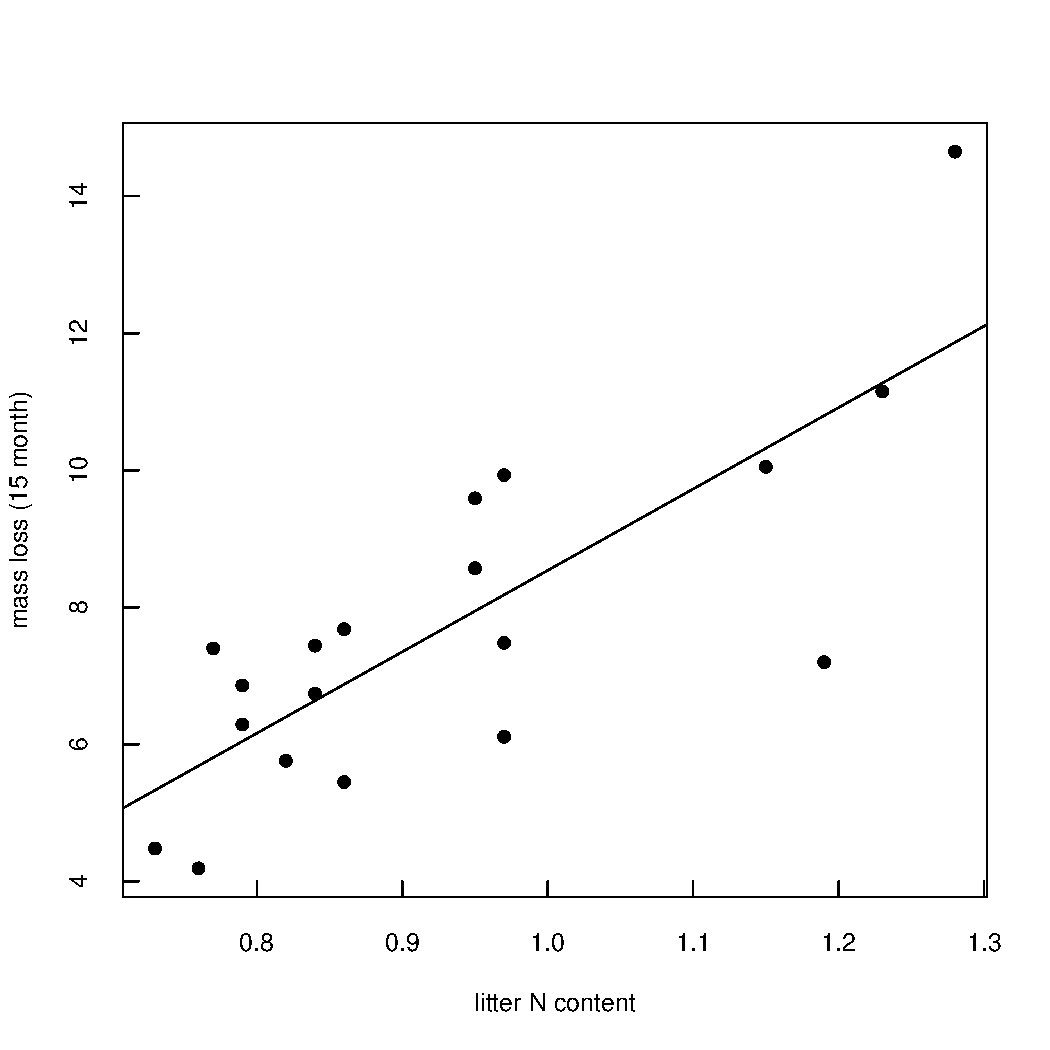
\includegraphics[width=8.3cm]{massloss_n_lit.pdf}
\end{center}
\label{n_massloss}
\caption{Litter mass loss after 15 month vs. litter N content. R= 0.795, p \textless .001}
\end{figure}

\begin{figure}[t]
\vspace*{2mm}
\begin{center}
\includegraphics[width=8.3cm]{resp_glcdepoly_h2.pdf}
\includegraphics[width=8.3cm]{resp_glcdepoly_h3.pdf}
\end{center}
\label{resp_depoly}
\caption{Quotient of respiration and glucan depolymerization. In AK microbial community respire significantly more non-glucose carbon after 2, but not after 6 month. Data from \cite{Leitner2011}}
\end{figure}

\begin{figure}[t]
\vspace*{2mm}
\begin{center}
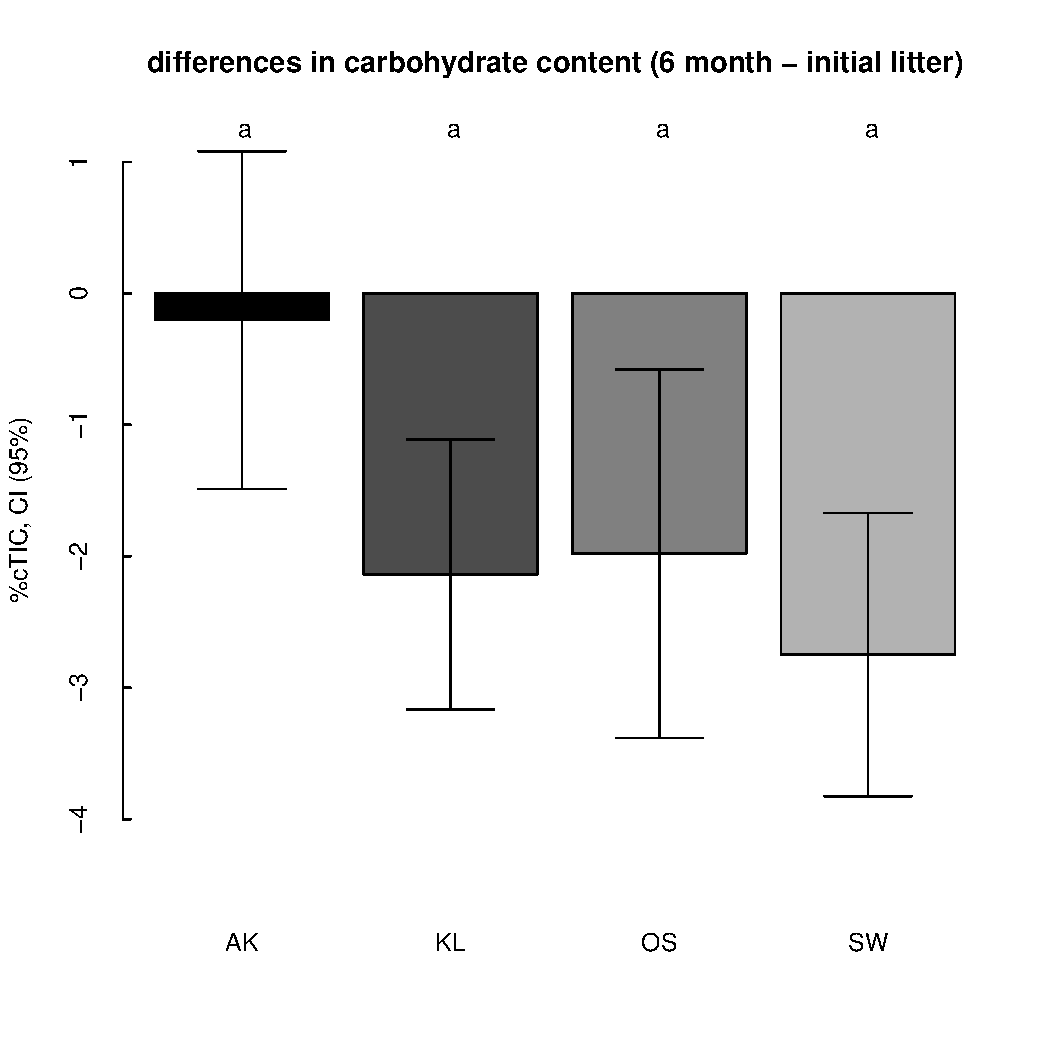
\includegraphics[width=8.3cm]{carb_differences_h3h0.pdf}
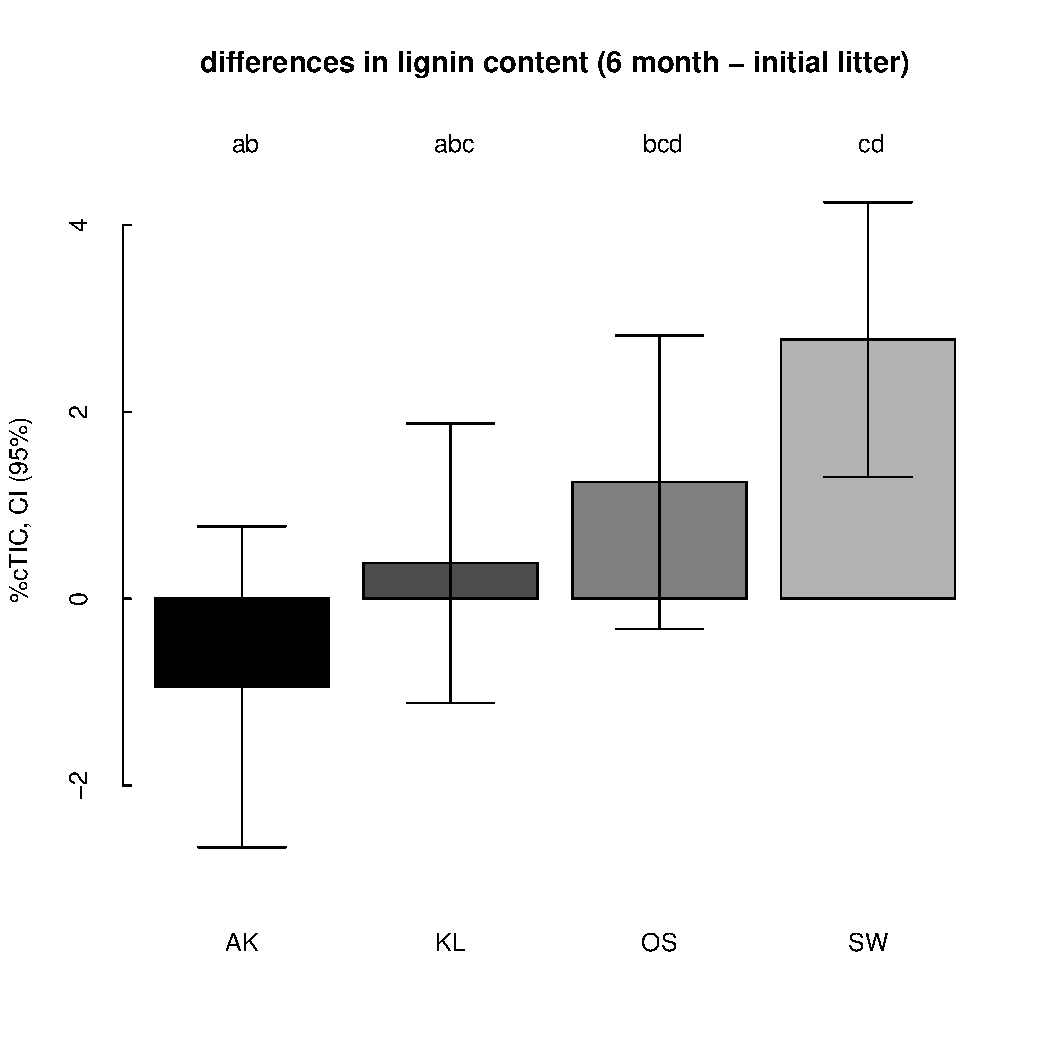
\includegraphics[width=8.3cm]{lig_differences_h3h0.pdf}
\end{center}
\label{car_lig_6month}
\caption{Difference in \% cTIC (sum of lig markers). error bars indicate 95\% confidence intervall.}
\end{figure}

\begin{figure}[t]
\vspace*{2mm}
\begin{center}
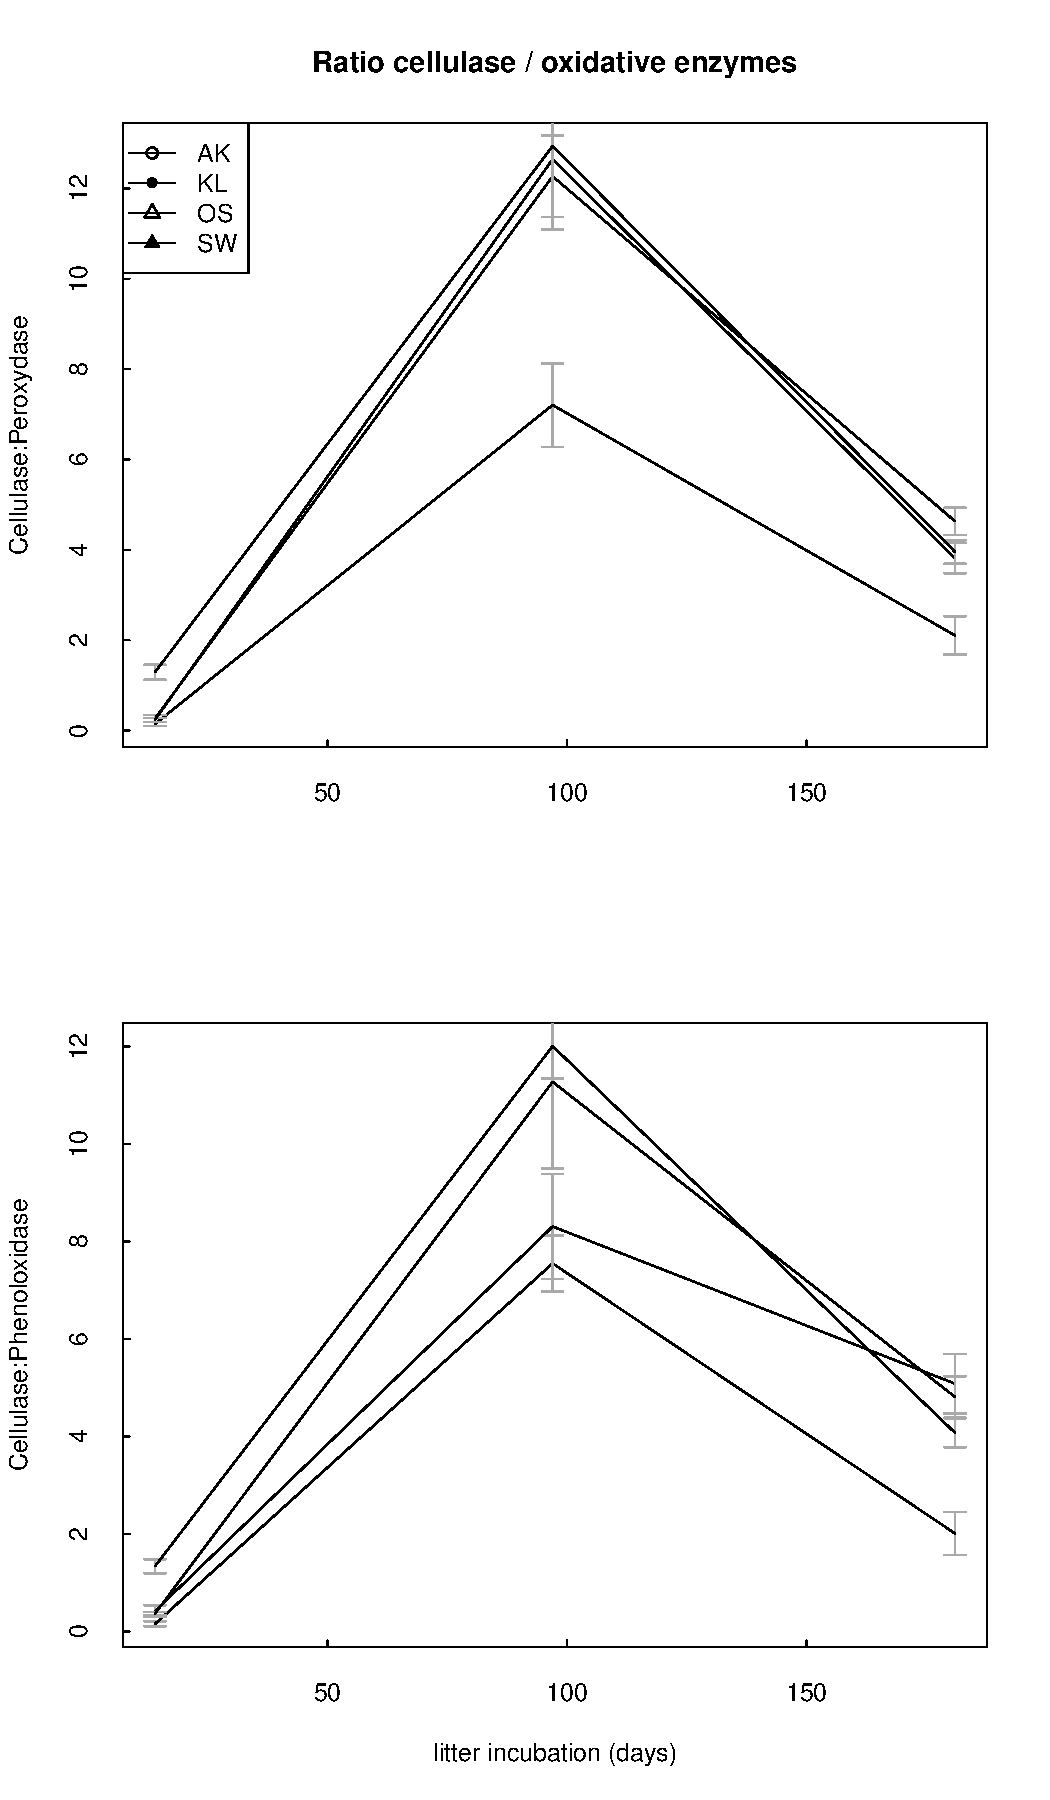
\includegraphics[width=8.3cm]{enzymeratio.pdf}
\end{center}
\label{enz_ratio}
\caption{Ratio between cellulase and two oxidative enzymes (phenolxydase and peroxydase). The two ratios are strongly correlated, oxidative enzymes are higher in AK than in other litter types.}
\end{figure}



\begin{figure*}[t]
\vspace*{2mm}
\begin{center}
%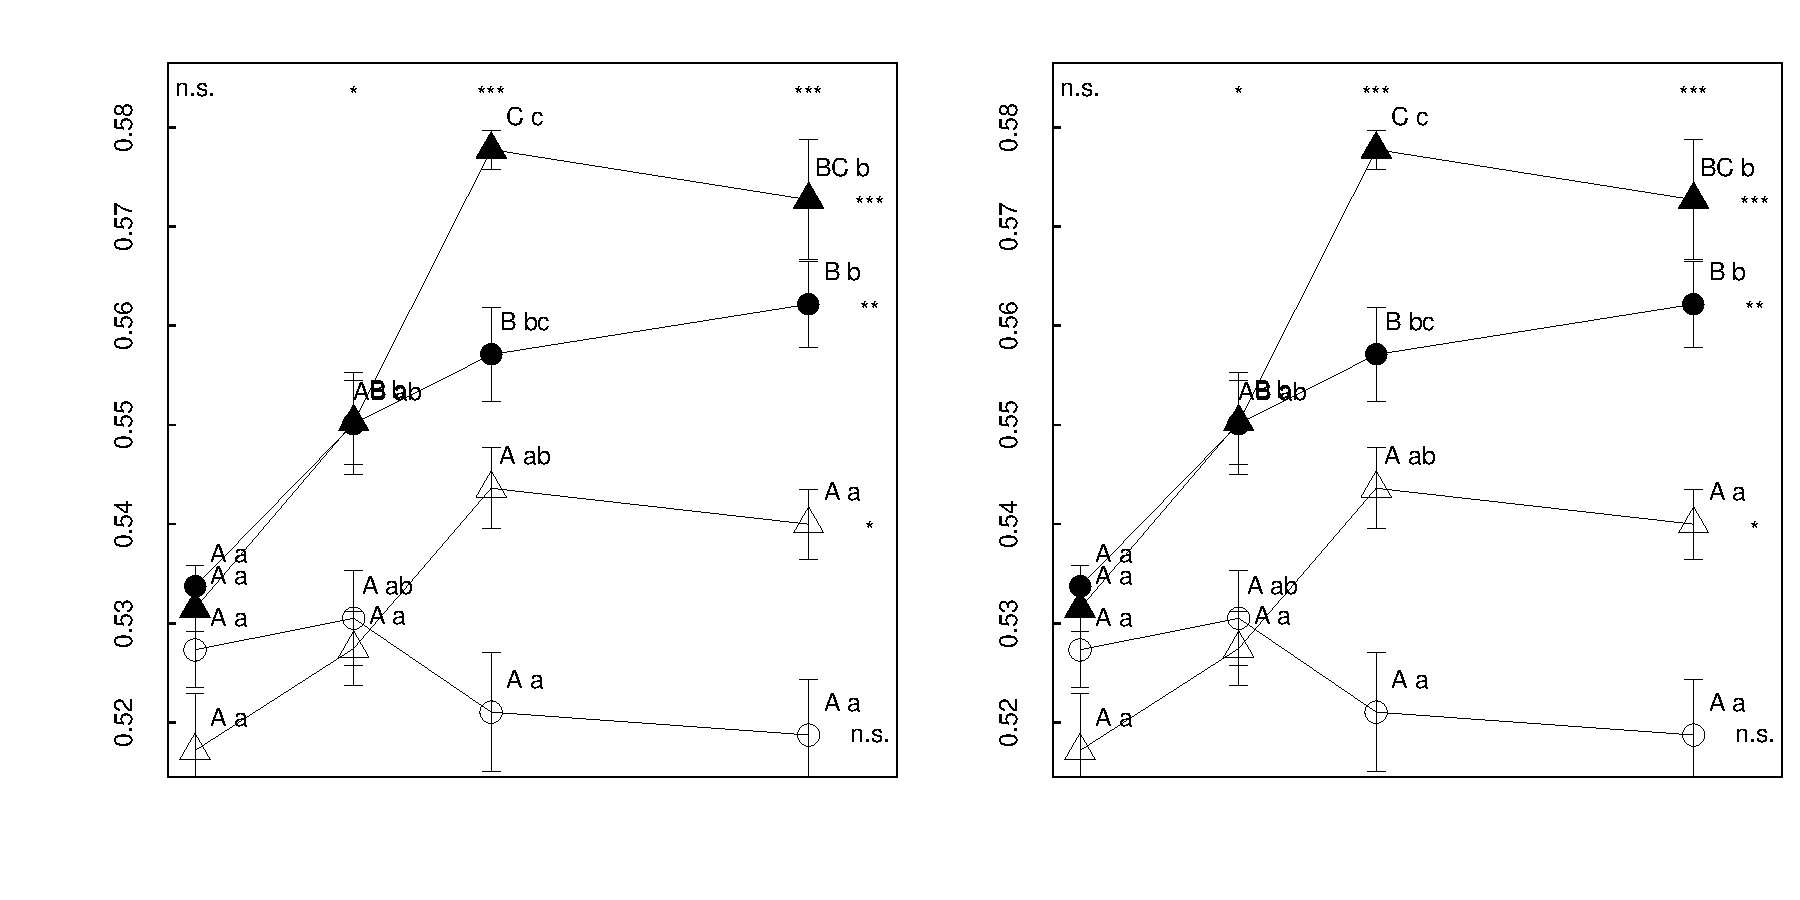
\includegraphics[width=12cm]{timeseries_lci.pdf}
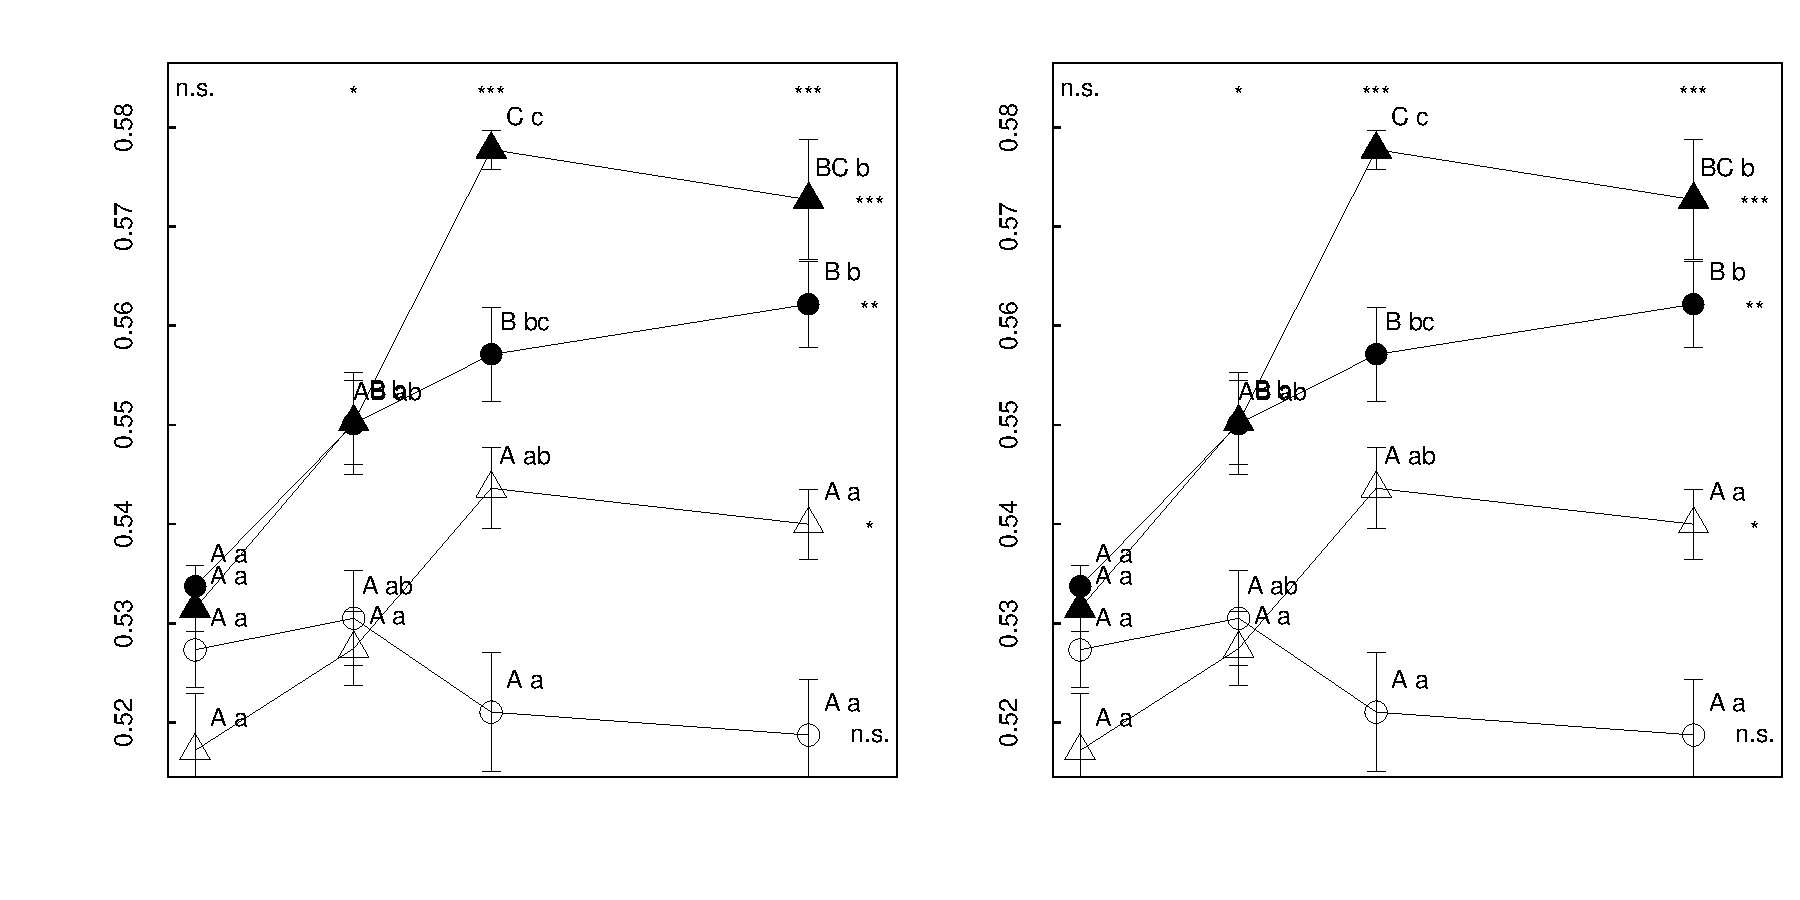
\includegraphics[width=17cm]{timeseries_lci.pdf}
\end{center}
\label{lci}
\caption{Development of the LCI (Lignin:(Lignin+Carbohydrates) and Lignin:N ratio}
\end{figure*}

\begin{figure}[t]
\vspace*{2mm}
  \begin{center}
%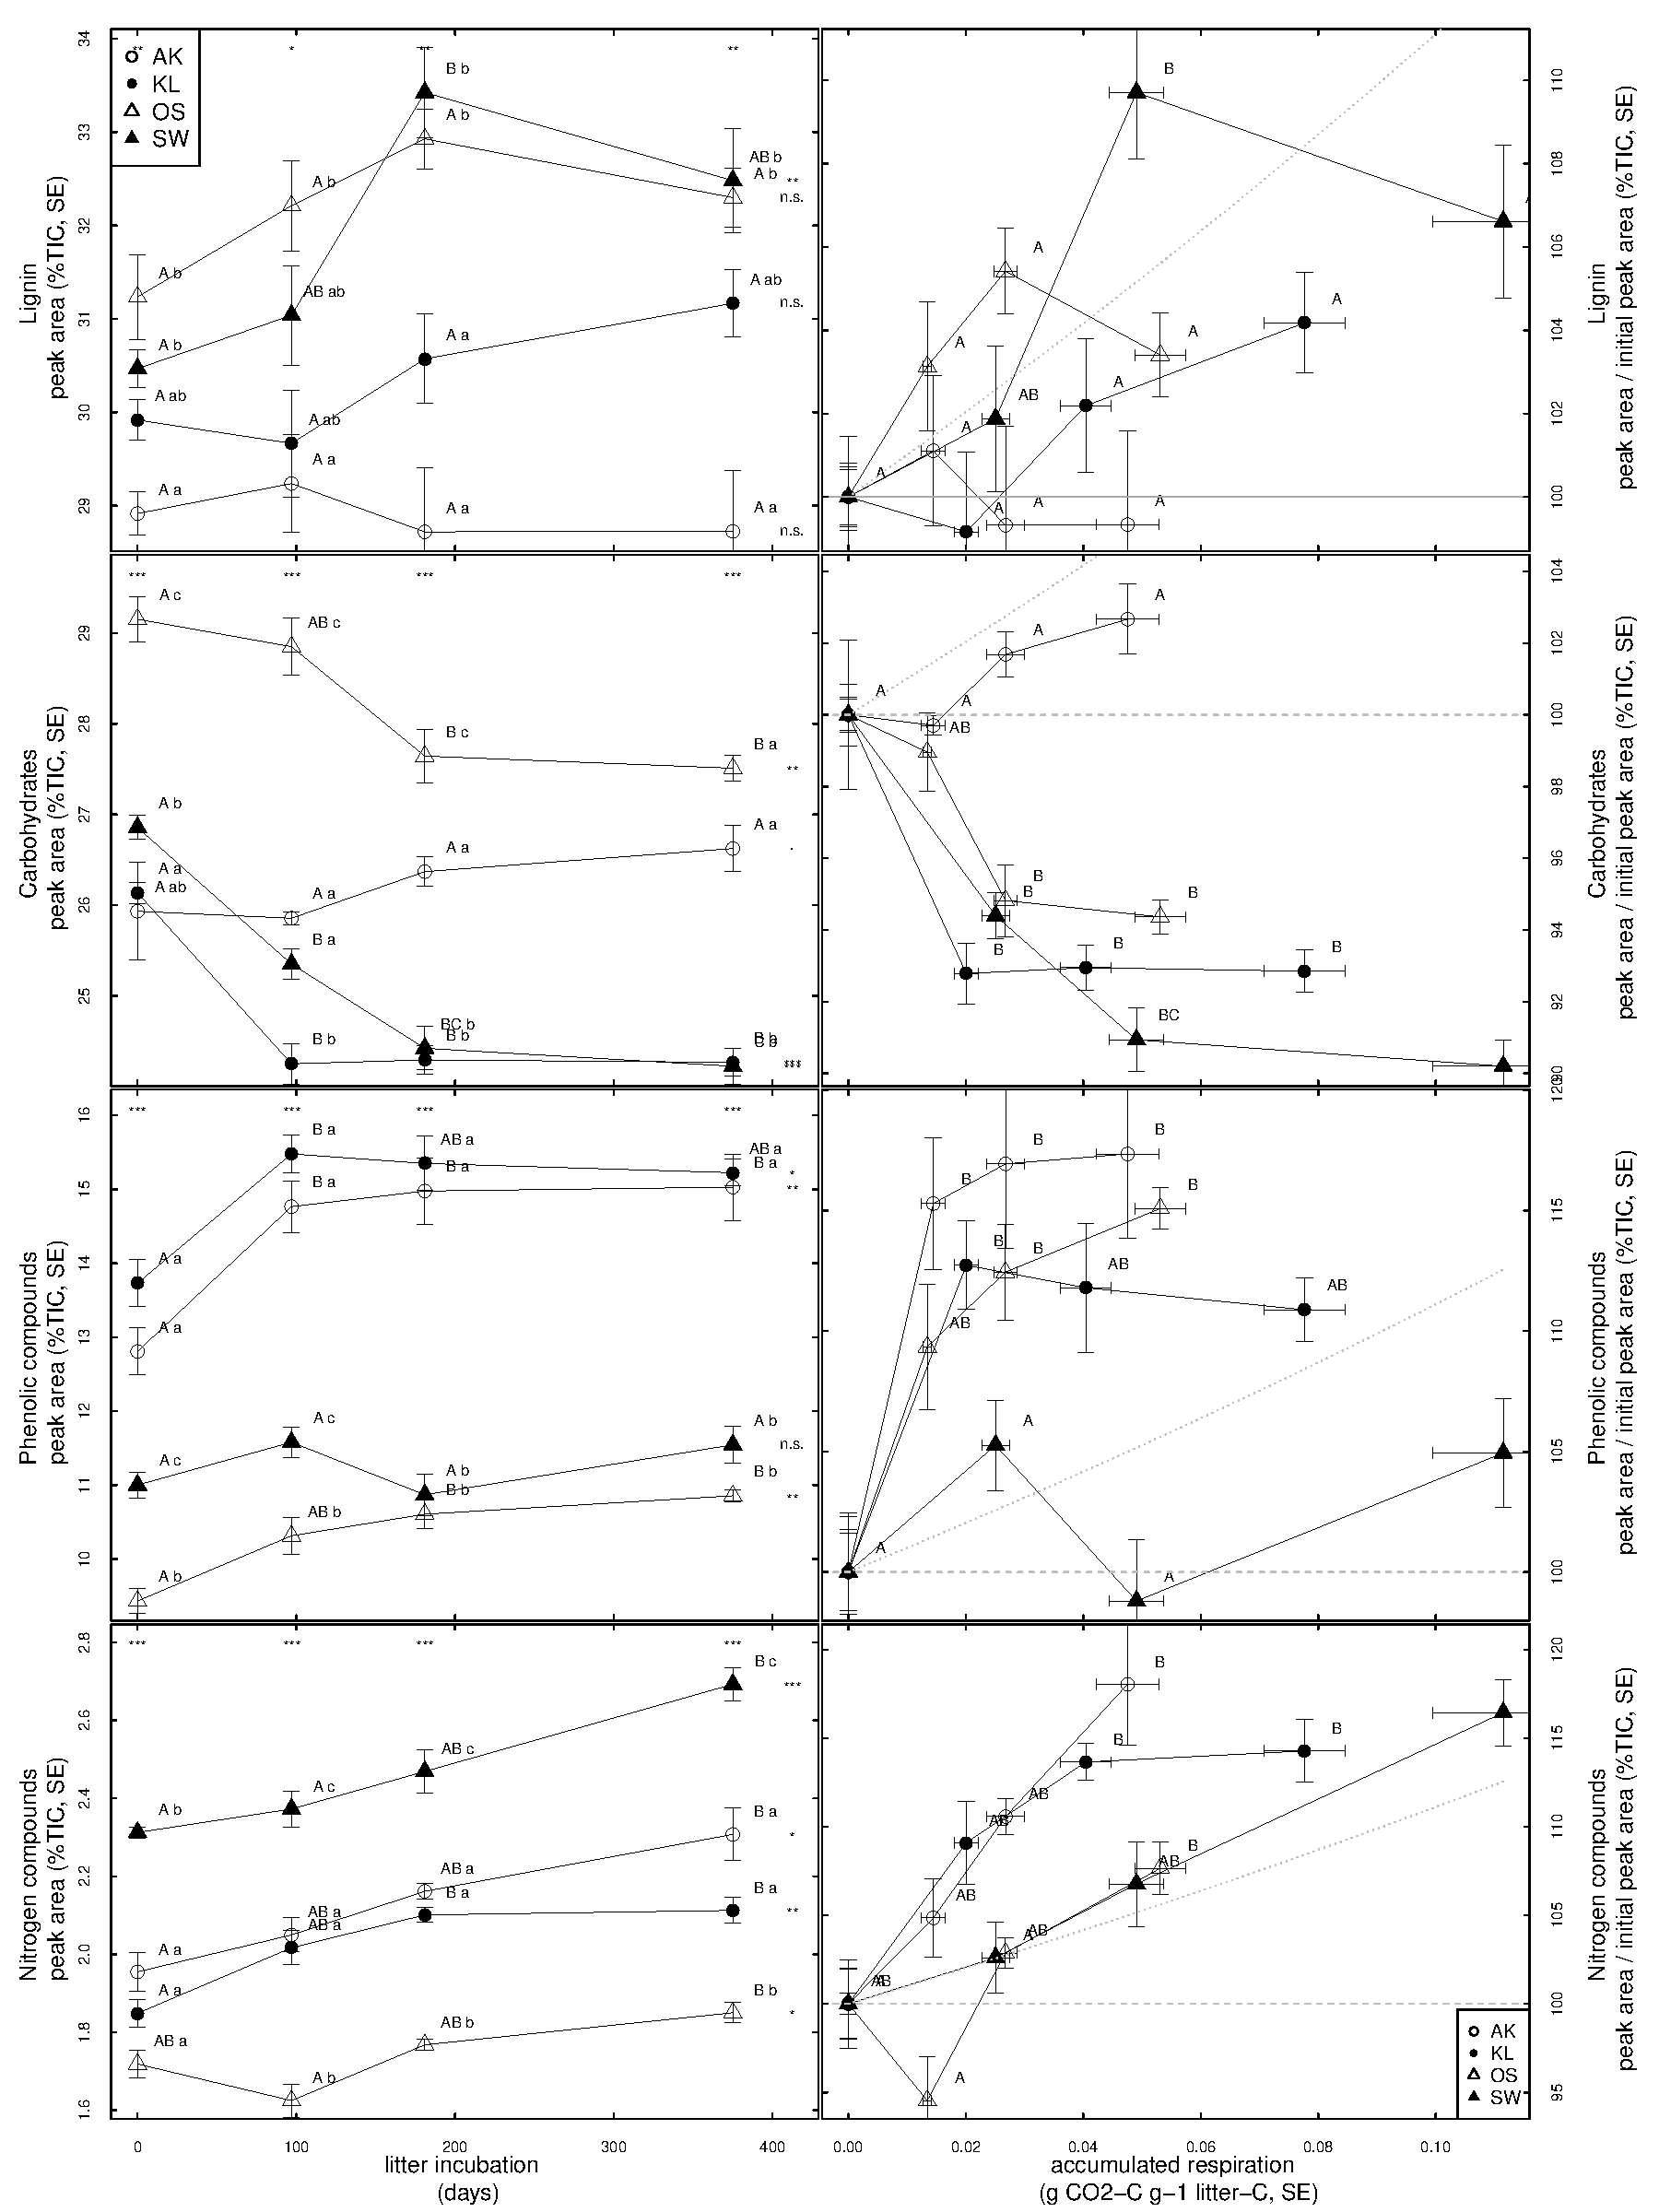
\includegraphics[width=12cm]{timeseries_orig.pdf}
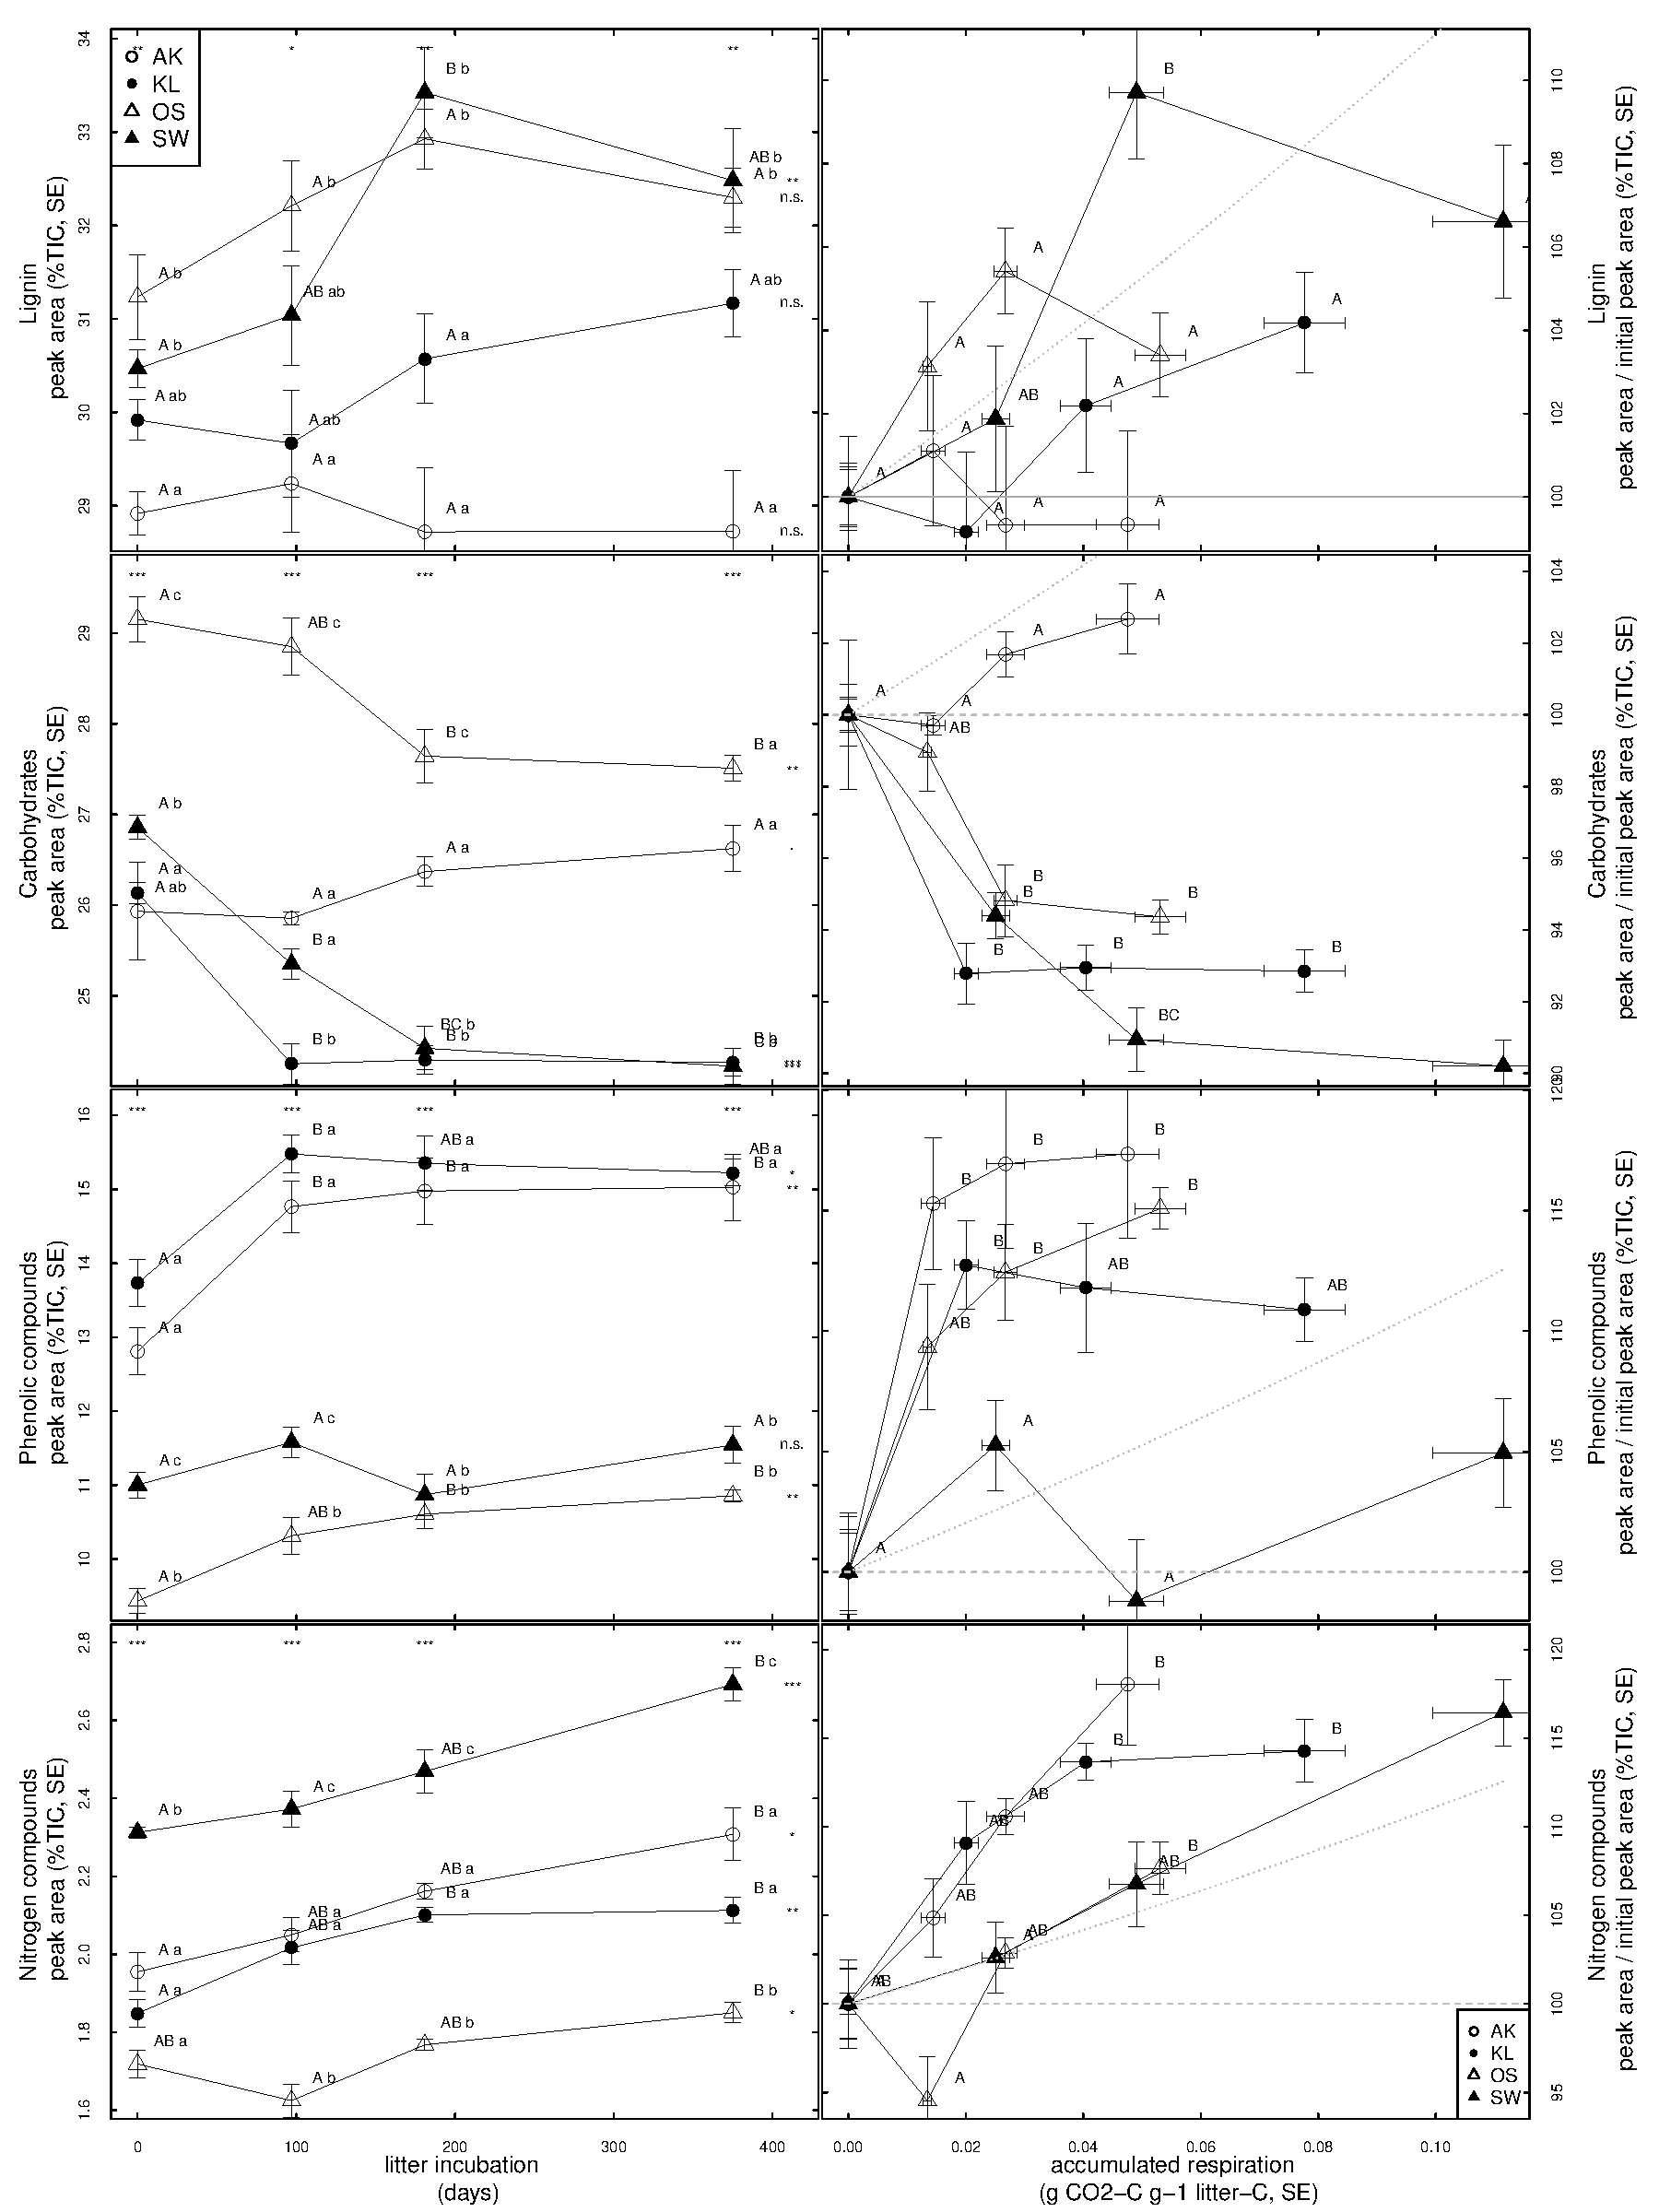
\includegraphics[width=17cm]{timeseries_orig.pdf}

\end{center}
\label{timeseries}
\caption{Decomposition dynamics of HMW compound classes}
\end{figure}


\begin{figure*}[t]
\vspace*{2mm}
\begin{center}
\includegraphics[width=12cm]{allpeaks_allharvests_PCA12.pdf}
\includegraphics[width=12cm]{allpeaks_allharvests_PCA34.pdf}

\end{center}
\caption{TEXT}
\end{figure*}


\begin{figure*}[t]
\vspace*{2mm}
\begin{center}
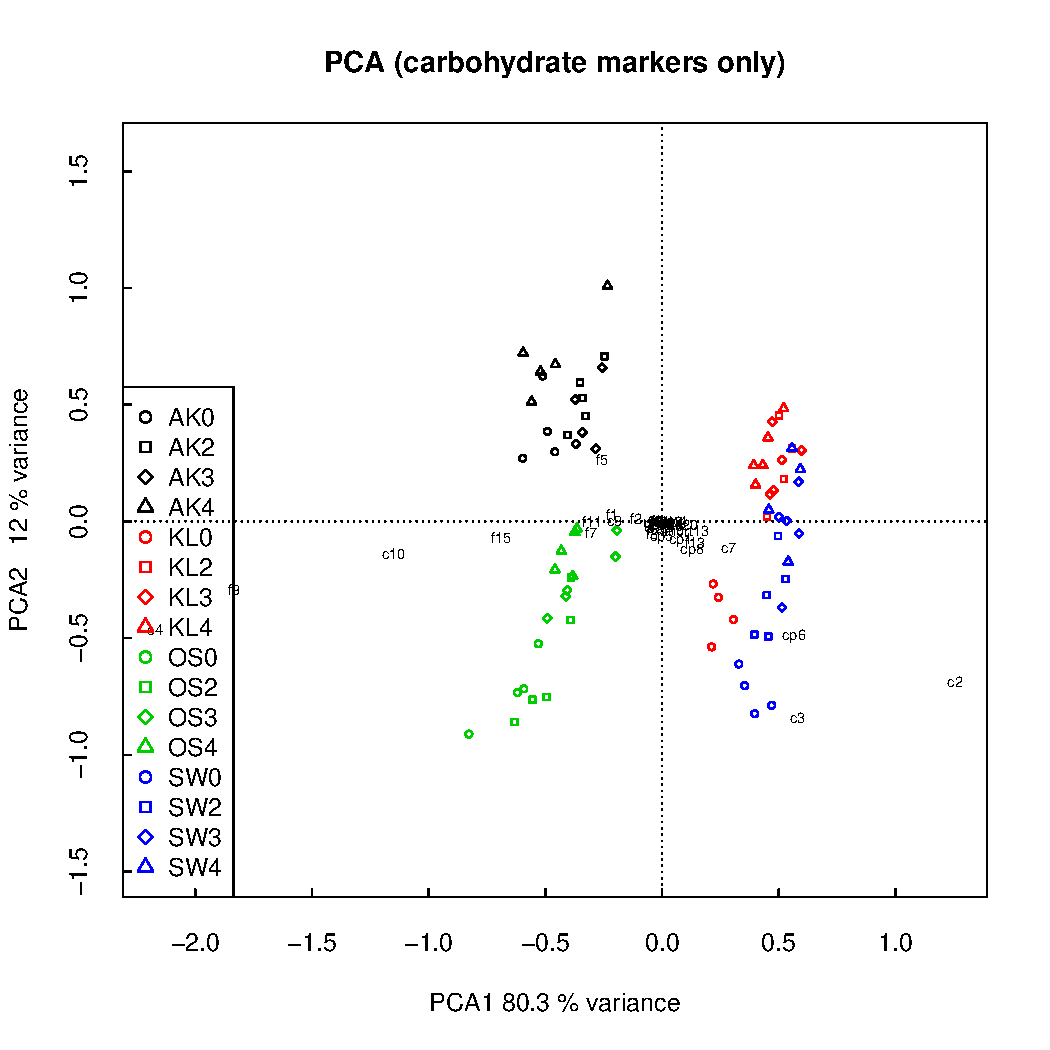
\includegraphics[width=12cm]{pca12_carbos.pdf}
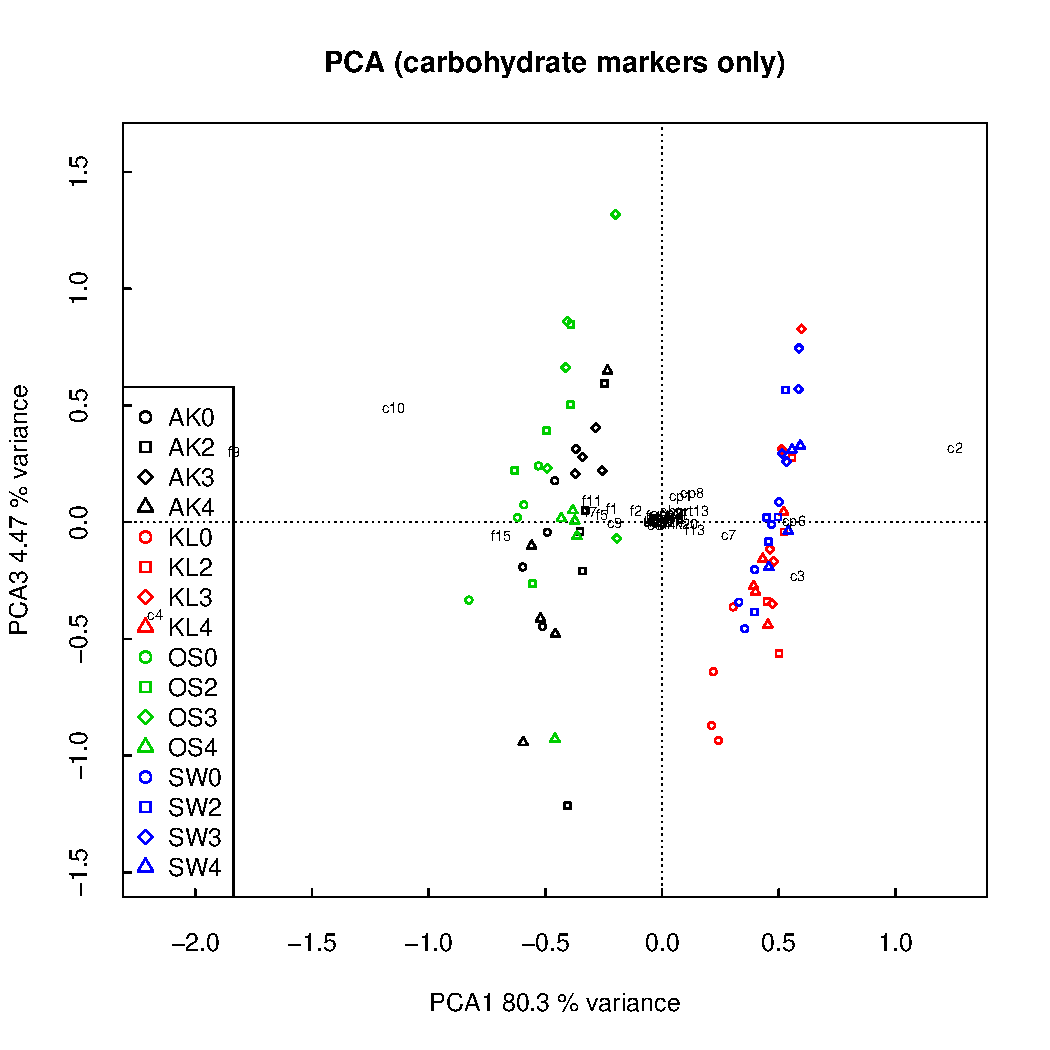
\includegraphics[width=12cm]{pca13_carbos.pdf}

\end{center}
\caption{TEXT}
\end{figure*}

%% TWO-COLUMN FIGURES

%f
\begin{figure*}[t]
\vspace*{2mm}
\begin{center}
\includegraphics[width=12cm]{ligonly_allharvests_PCA12.pdf}
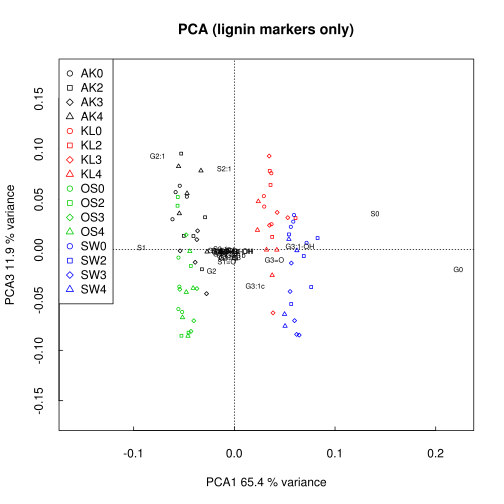
\includegraphics[width=12cm]{ligonly_allharvests_PCA13.pdf}

\end{center}
\caption{TEXT}
\end{figure*}


\begin{figure*}[t]
\vspace*{2mm}
\begin{center}
\includegraphics[width=12cm]{controls_h1.pdf}
\end{center}
\label{litchem_h1}
\caption{Litter chemistry: content of macro and micronutrients, 14 days after innoculation, n=5}
\end{figure*}

\begin{figure*}[t]
\vspace*{2mm}
\begin{center}
\includegraphics[width=12cm]{controls_h2.pdf}
\end{center}
\label{litchem_h2}
\caption{Litter chemistry: content of macro and micronutrients, 97 days after innoculation, n=5}
\end{figure*}

\begin{figure*}[t]
\vspace*{2mm}
\begin{center}
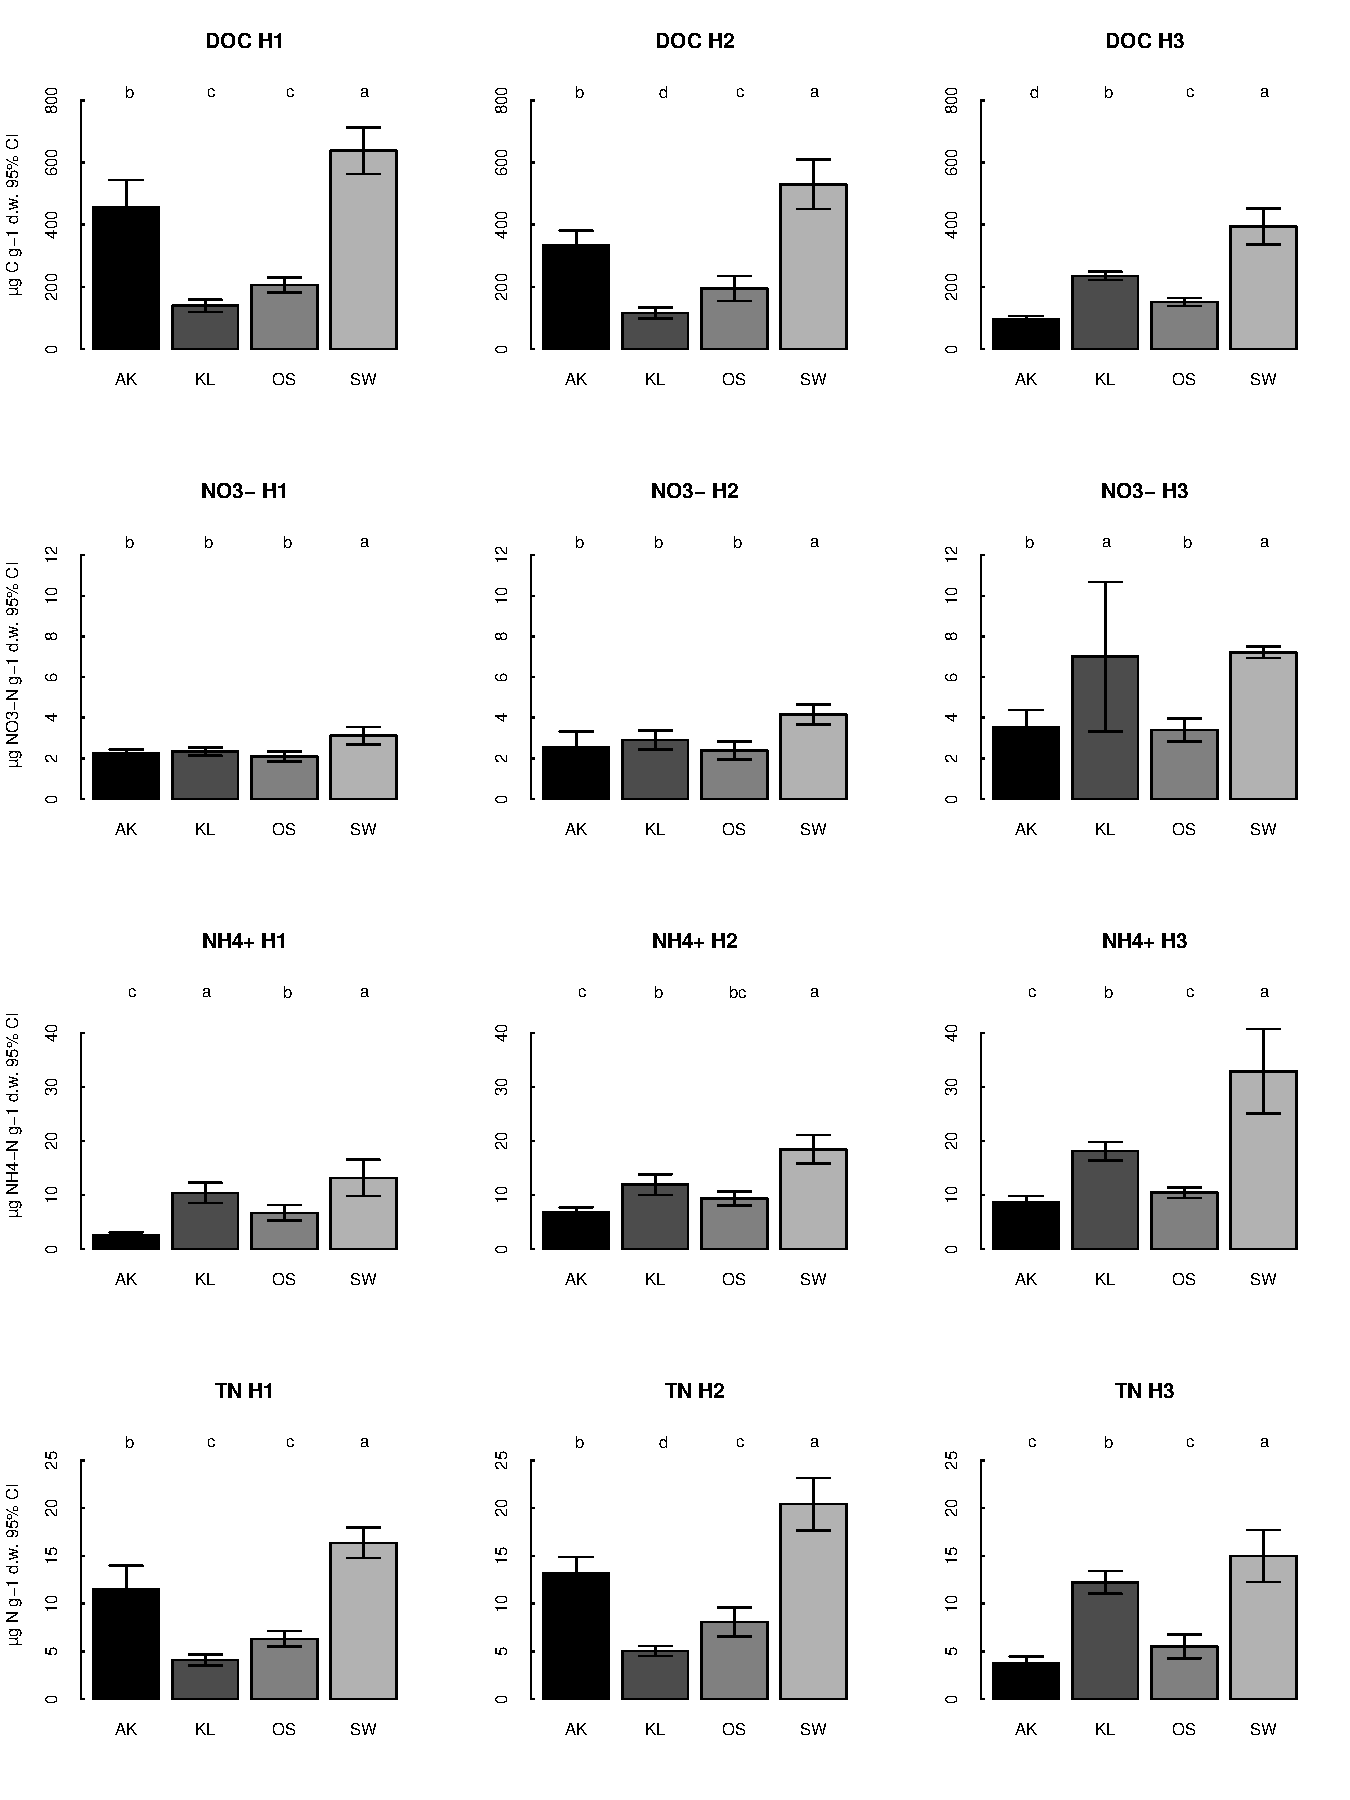
\includegraphics[width=12cm]{doc_barplots.pdf}
\end{center}
\label{doc}
\caption{dissolved organic carbon, total dissolved nitrogen, no3-, nh4+}
\end{figure*}

\begin{figure*}[t]
\vspace*{2mm}
\begin{center}
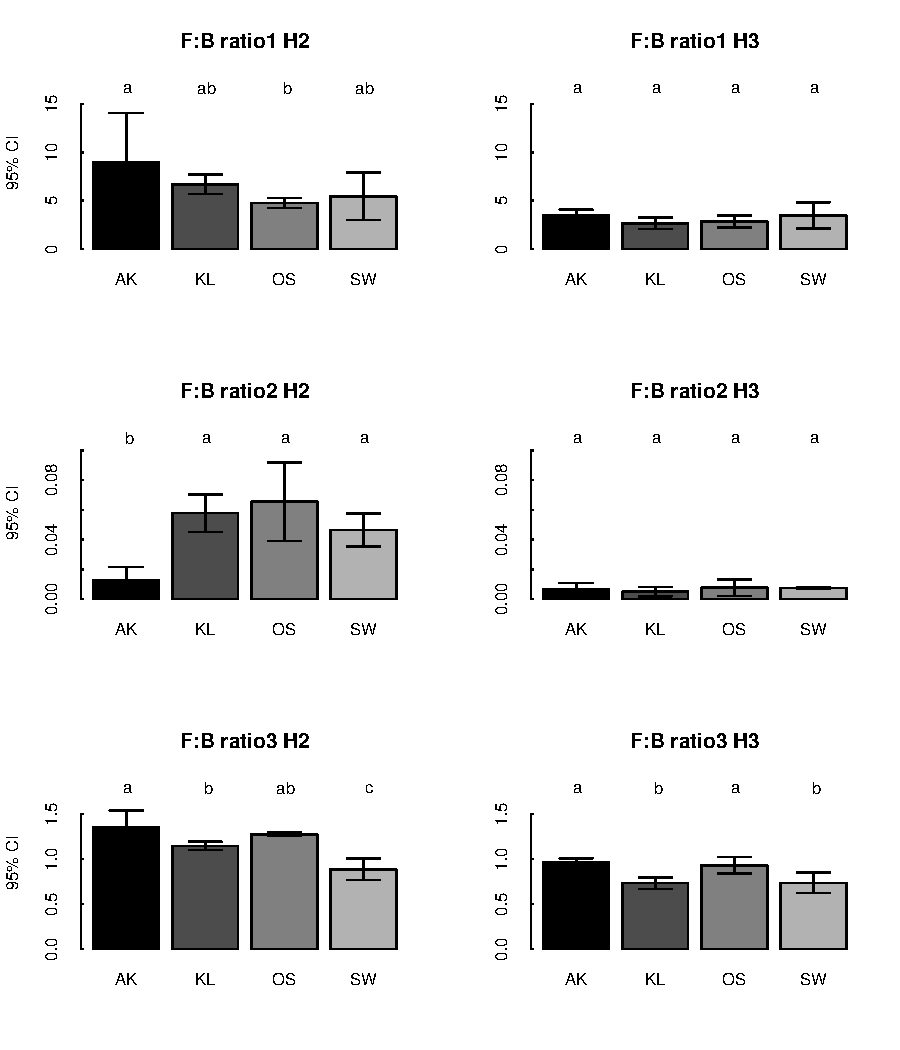
\includegraphics[width=12cm]{plfa.pdf}
\end{center}
\label{plfa}
\caption{Fungi : Bacteria ratios}
\end{figure*}


%% TABLES %%%%%%%%%%%%%%%%%%%%%%%%%%%%%%%%%%%%%%%%%%%%%%%%%%%%%%%%%%%%%%%%%%%%


%% ONE-COLUMN TABLE
%t
%\begin{table}[t]
%\caption{TEXT}
%\vskip4mm
%\centering
%\begin{tabular}{lllrr}
%\tophline
%
%\middlehline
%
%\bottomhline
%\end{tabular}
%\end{table}


%% TWO-COLUMN TABLE

%t
%\begin{table*}[t]
%\caption{TEXT}
%\vskip4mm
%\centering
%\begin{tabular}{lllrr}
%\tophline
%
%\middlehline
%
%\bottomhline
%\end{tabular}
%\end{table*}

%t
\begin{table*}[t]
\caption{TEXT}
\vskip4mm
\centering
\begin{tabular}{lllll}
\tophline
Substance&code&origin&RT&m/z integrated\\
\middlehline
Furan&C&C&2.35&39+68\\ 
Methylfuran&C&C&2.74&81+82\\ 
Methylfuran&C&C&2.91&81+82\\ 
Dimethylfuran&C&C&3.43&95+96\\ 
Dimethylfuran&C&C&3.66&95+96\\ 
Vinylfuran&C&C&5.01&65+94\\ 
3-Furaldehyd&C&C&11.57&95+96\\ 
2(5H)Furanon&C&C&11.69&55+98\\ 
2-Furaldehyd&C&C&12.22&95+96\\ 
Acetylfuran&C&C&12.99&95+110\\ 
5-Methyl-2-furancarboxaldehyde&C&C&14.23&109+110\\ 
Butyrolactone&C&C&15.22&56+86\\ 
Furanmethanol&C&C&15.61&98\\ 
5-Methyl-2(5H)-furanone&C&C&16.06&55+98\\ 
5-hydroxymethylfuran-1-carboxaldehyde&C&C&27.51&97+126\\ 
%unknown_furan_6.36&C&C&NA&\\ 
%10.26_2-cyclopenten-1-one&C&C&10.26&53+54+52\\ 
%10.51_2-methyl-2-cyclopenten-1-one&C&C&10.51&53+96\\ 
%13.31_3-methyl-cyclopentanone&C&C&13.31&67+96\\ 
%13.69_dimethylcyclopentenone&C&C&13.69&67+95+110\\ 
%14.44_2-cyclopenten-1&4-dione&C&C&14.44&54+68+96\\ 
%17.51_1&2-cylopentandione&C&C&17.51&55+98\\ 
%18.14_2-cyclopenten-1-one&_-2-hydroxy-3-me&C&C&18.14&98\\ 
%18.42_1&2-cyclopentanedione&_-3-methyl-&C&C&18.42&69+112\\ 

%2-Oxopropanoic Acid& ME&C&C&7.92&43+102\\ 
1-Hydroxypropanone&C&C&9.24&43\\ 
%Propanoic acid& ME&C&C&12.1&43+102\\ 
unknown carbohydrate 1&C&C&19.06&58+86+114\\ 
unknown carbohydrate 2&C&C&19.35&98+126\\ 
unknown carbohydrate 3&C&C&21.77&116\\ 
unknown carbohydrate 4&C&C&22.33&44\\ 
unknown carbohydrate 5&C&C&26.18&57+69\\ 
unknown carbohydrate 6&C&C&31.67&73+135\\ 
laevoglucosan&C&C&40.44&60+73\\ 
27:1&Cut&Cut&NA&\\ 
29:0&Cut&Cut&NA&\\ 
29:1&Cut&Cut&NA&\\ 
G0&L&L&18.87&109+124\\ 
G1&L&L&20.32&123+138\\ 
G2&L&L&21.4&137+152\\ 
G3:1a&L&L&23.29&149+164\\ 
G2:1&L&L&23.69&135+150\\ 
G3:1b&L&L&24.48&149+164\\ 
S0&L&L&24.58&139+154\\ 
G3:1c&L&L&25.66&149+164\\ 
S1&L&L&25.67&153+168\\ 
S2&L&L&26.39&167+182\\ 
H3:1&L&L&27.76&133+134\\ 
S3:1a&L&L&27.97&179+194\\ 
S2:1&L&L&28.37&165+180\\ 
G1=O&L&L&28.4&109+152\\ 
G3&L&L&28.72&137+166\\ 
G3=O/-OH&L&L&28.77&182\\ 
S3:1b&L&L&28.91&179+194\\ 
G2=O&L&L&29.2&151+166\\ 
G3=O&L&L&29.36&137+180\\ 
S3:1c&L&L&30.16&194+179\\ 
S1=O&L&L&32.68&139+182\\ 
H1=O&L&L&32.7&121+122\\ 
S3=O/-OH&L&L&32.8&212\\ 
GAc&L&L&32.88&137+182\\ 
S3&L&L&33.15&181+196\\ 
S3=O&L&L&33.32&167+210\\ 
G3:1=O&L&L&35.3&135+178\\ 
G3:1-OH&L&L&37.1&180\\ 
SAc&L&L&38.78&212\\ 
S3:1=O&L&L&43.06&165+208\\ 
toluene&N&N&NA&\\ 
N-methyl-pyrrol&N&N&NA&\\ 
pyridine&N&N&NA&\\ 
methylpyridine1&N&N&NA&\\ 
methylpyridine2&N&N&NA&\\ 
pyrrole&N&N&NA&\\ 
methylpyrrol1&N&N&NA&\\ 
methylpyrrol2&N&N&NA&\\ 
Pyridol&N&N&NA&\\ 
Indole&N&N&NA&\\ 
Methylindole&N&N&NA&\\ 
%methylpyridine3_7.54&N&N&NA&\\ 
xylene1&non&non&NA&\\ 
xylene2&non&non&NA&\\ 
xylene3&non&non&NA&\\ 
methoxymethylbenzene&non&non&NA&\\ 
benzaldehyde&non&non&NA&\\ 
1-Methyl-4-methoxybenzene&non&non&15.98&\\ 
Aceton&non&non&2.46&\\ 
2-Propenal&non&non&2.6&\\ 
2-Butanal&non&non&4.56&\\ 
2,3-Pentadione&non&non&4.77&\\ 
Hexanal&non&non&5.16&\\ 
1-Penten-3-one&non&non&11.28&\\ 
&Ph&Ph&21.02&\\ 
&Ph&Ph&22.11&\\ 
&Ph&Ph&22.22&\\ 
&Ph&Ph&23.38&\\ 
&Ph&Ph&26.93&\\ 
&Ph&Ph&31.11&\\ 
&Ph&Ph&31.86&\\ 
&Ph&Ph&33.4&\\ 
%unknown_alcyl_20.00&al&al&NA&\\ 
%xylene4_6.99&non&non&NA&\\ 
%limonen_7.29&non&non&NA&\\ 
%indene_12.64&non&non&NA&\\ 

% unknown_20.85&unk&unk&NA&\\ 
% unknown_20.86&unk&unk&NA&\\ 
% unknown_22.43&unk&unk&NA&\\ 
% unknown_alkyl_22.82&unk&unk&NA&\\ 
% hexan2&4dione&_-enol_23.92&unk&unk&NA&\\ 
% benzofuran_26.19&unk&unk&NA&\\ 
% unknown_27.76&unk&unk&NA&\\ 
% 3-Penten-2-one&non&non&3.89&\\ 
% 2,3-Butandione&non&non&3.67&\\ 
% 3-Buten-2-one&non&non&3.39&\\ 
% Methanol&non&non&2.88&\\ \bottomhline
\end{tabular}
\end{table*}


%% The different columns must be seperated with a & command and should
%% end with \\ to identify the column brake.

%%%%%%%%%%%%%%%%%%%%%%%%%%%%%%%%%%%%%%%%%%%%%%%%%%%%%%%%%%%%%%%%%%%%%%%%%%%%%%


%% If figures and tables must be numbered 1a, 1b, etc. the following command
%% should be inserted before the begin{} command.

%\addtocounter{figure}{-1}\renewcommand{\thefigure}{\arabic{figure}a}


\end{document}
